\documentclass{article}

\usepackage[top=3cm, bottom=3cm, left=3cm,right=3cm]{geometry}
\usepackage[colorinlistoftodos]{todonotes}
\usepackage{graphicx}
\usepackage{amssymb}
\usepackage{amsmath}
\usepackage{bbm}
\usepackage{todonotes}
\usepackage{pdflscape}
\usepackage{caption}
\usepackage{subcaption}
\usepackage[T1]{fontenc}
\usepackage[utf8]{inputenc}
\usepackage{authblk}
\usepackage{array}
\usepackage{multirow}
\usepackage{pdfpages}
\usepackage{setspace} 
\usepackage{booktabs}
\usepackage{longtable}
\usepackage{float}
\usepackage{tikz}
\usepackage{pifont}
\usepackage[colorlinks=true,citecolor=blue, linkcolor=blue]{hyperref}
\usepackage{multirow}
\setlength{\tabcolsep}{5pt}
%%\setlength{\parindent}{0pt}
\usepackage[parfill]{parskip}
\renewcommand{\arraystretch}{1.5}

\renewcommand\Affilfont{\itshape\footnotesize}
\def\ci{\perp\!\!\!\perp}

% bibliography
\renewcommand\Affilfont{\itshape\footnotesize}
\linespread{1.5}
\newcolumntype{C}[1]{>{\centering\let\newline\\\arraybackslash\hspace{0pt}}m{#1}}

% \usepackage{lineno}
% \linenumbers

% Nature Bibliography style
\usepackage[backend=biber,style=nature]{biblatex}
\addbibresource{library.bib} 

\newcommand{\xmark}{\ding{55}}

%%%%%%%%%%%%%
%%% Title %%%
%%%%%%%%%%%%%
\title{Supplementary Material: District-level male medical and traditional circumcision coverage and unmet need in sub-Saharan Africa}

\author{}
\date{}

%%%%%%%%%%%%%%%%%%%%%%%%%%%%%%%%%%%%%%%%%%%%%%%%%%%%%%%%%%%%%%%%%%
%%%%%%%%%%%%%%%%%%%%%%%%%%%%%%%%%%%%%%%%%%%%%%%%%%%%%%%%%%%%%%%%%%
%%%%%%%%%%%%%%%%%%%%%%%%%%%%%%%%%%%%%%%%%%%%%%%%%%%%%%%%%%%%%%%%%%

\begin{document}

%%%%%%%%%%%%%%%%%%%%%%%%%%%%%%%%%%%%%%%%%%%%%%%%%%%%%%%%%%%%%%%%%%
%%%%%%%%%%%%%%%%%%%%%%%%%%%%%%%%%%%%%%%%%%%%%%%%%%%%%%%%%%%%%%%%%%
%%%%%%%%%%%%%%%%%%%%%%%%%%%%%%%%%%%%%%%%%%%%%%%%%%%%%%%%%%%%%%%%%%

\maketitle

\vspace{-1cm}

Patrick O'Toole\textsuperscript{1},
Matthew L. Thomas\textsuperscript{1,2},
Oliver Stevens\textsuperscript{1},
Kevin Lam\textsuperscript{1,3},
Katharine Kripke\textsuperscript{4},
Rachel Esra\textsuperscript{1},
Ian Wanyeki\textsuperscript{5},
Lycias Zembe\textsuperscript{5},
Jeffrey W. Eaton\textsuperscript{1,6} \\
\smallskip
  
\textbf{1} MRC Centre for Global Infectious Disease Analysis, School of Public Health, Imperial Colleg  e London, London, United Kingdom\\
\textbf{2} Department of Earth and Environmental Sciences, University of Manchester, Manchester, United Kingdom\\
\textbf{3} Department of Statistics, University of British Columbia, Vancouver, Canada\\
\textbf{4} Avenir Health, Washington, District of Columbia, United States of America\\
\textbf{5} Joint United Nations Programme on HIV/AIDS (UNAIDS), Geneva, Switzerland\\
\textbf{6} Center for Communicable Disease Dynamics, Department of Epidemiology, Harvard T.H. Chan School of Public Health, Boston, Massachusetts, United States of America\\

\smallskip

* Corresponding Author Email

\newpage

%%%%%%%%%%%%%%%%%%%%%%%%%%%%%%%%%%%%%%%%%%%%%%%%%%%%%%%%%%%%%%%%%%
%%%%%%%%%%%%%%%%%%%%%%%%%%%%%%%%%%%%%%%%%%%%%%%%%%%%%%%%%%%%%%%%%%
%%%%%%%%%%%%%%%%%%%%%%%%%%%%%%%%%%%%%%%%%%%%%%%%%%%%%%%%%%%%%%%%%%

\begin{appendix}

%%%%%%%%%%%%%%%%%%%%%%%%%%%%%%%%%%%%%%%%%%%%%%%%%%%%%%%%%%
%%%% Resetting figure and table count for the appendix %%%
%%%%%%%%%%%%%%%%%%%%%%%%%%%%%%%%%%%%%%%%%%%%%%%%%%%%%%%%%%
%\setcounter{figure}{0} \renewcommand{\thefigure}{A.\arabic{figure}}
%\setcounter{table}{0} \renewcommand{\thetable}{A.\arabic{table}}

\newpage

\tableofcontents

\newpage

%%%%%%%%%%%%%%%%%%%%%%%%%%%%%%%%%%%%%%%%%%%%%%%%%%%%%%%%%%%%%%%%%%
%%%%%%%%%%%%%%%%%%%%%%%%%%%%%%%%%%%%%%%%%%%%%%%%%%%%%%%%%%%%%%%%%%
%%%%%%%%%%%%%%%%%%%%%%%%%%%%%%%%%%%%%%%%%%%%%%%%%%%%%%%%%%%%%%%%%%

\section{Data}
\label{sec:org8802288}

%%%%%%%%%%%%%%%%%%%%%%%%%%%%%%%%%%%%%%%%%%%%%%%%%%%%%%%%%%%%%%%%%%
%%%%%%%%%%%%%%%%%%%%%%%%%%%%%%%%%%%%%%%%%%%%%%%%%%%%%%%%%%%%%%%%%%
%%%%%%%%%%%%%%%%%%%%%%%%%%%%%%%%%%%%%%%%%%%%%%%%%%%%%%%%%%%%%%%%%%

\subsection{Survey Data}
\label{sec:org09db5e8}

%%%%%%%%%%%%%%%%%%%%%%%%%%%%%%%%%%%%%%%%%%%%%%%%%%%%%%%%%%%%%%%%%%
%%%%%%%%%%%%%%%%%%%%%%%%%%%%%%%%%%%%%%%%%%%%%%%%%%%%%%%%%%%%%%%%%%

The study consisted of 33 sub-Saharan countries, that have conducted surveys that contained information on self-reported circumcision status since 2002: Senegal, Gambia, Guinea, Sierra Leone, Liberia, Mali, Burkina Faso, Côte d’Ivoire, Ghana, Togo, Benin, Niger, Nigeria, Cameroon, Chad, Ethiopia, Gabon, The Republic of the Congo (the Congo), The Democratic Republic of the Congo (DR Congo), Uganda, Kenya, Rwanda, Burundi, Tanzania, Angola, Zambia, Malawi, Mozambique, Zimbabwe, Namibia, Eswatini, Lesotho, South Africa. 
We excluded Equitorial Guinea, Guinea-Bissau, the Central African Republic and Botswana because they either had no surveys conducted, or, where surveys were available, there was insufficient information available on age at circumcision.  
In total, we identified 109 nationally representative household surveys conducted the study region between 2002 and 2019. These included several major survey series, namely the Demographic and Health Surveys (DHS), AIDS Indicator Surveys (AIS) Population-based HIV Impact Assessment (PHIA) surveys, Multiple Indicator Cluster Surveys (MICS), and, in the case of South Africa, Human Sciences Research Council (HSRC) surveys \cite{dhs, ais, phia, hsrc2002, hsrc2008, hsrc2012, hsrc2017} \todo{include MICS reference}.
Data on self-reported circumcision status were available in 104 out of the total 109 surveys. 
\textbf{[Expand on reasons for exclusions]} \textbf{[Link in your survey figure]} \todo{done, what do you mean by "link in survey figure?"}
Excluded surveys lacked information on age at circumcision, which made it impossible to make inferences on circumcision under our time-to-event modelling framework. The surveys which were excluded on the basis of this requirement were the 2008 Botswana AIDS Impact Survey (BAIS) and 2013 BAIS surveys, the Central African Republic 2018 MICS survey and the 2014 and 2018 Guinea-Bissau MICS surveys \cite{bais2008, bais2013}.
For 5 countries, namely Liberia, Senegal, Niger, Guinea, and the DR Congo, information on circumcision type was not available in any surveys. Therefore, only MC could be estimated in these countries, and no inferences about circumcision type, whether MMC or TMC, could be made.
See figure 1 for a visual representation of the different survey providers for each country, as well as the sample size of each survey and the availability of circumcision type information. 
See table 1 for the full list of surveys for each country, and the circumcision information included in each survey. 

\begin{figure}[H]
    \centering
    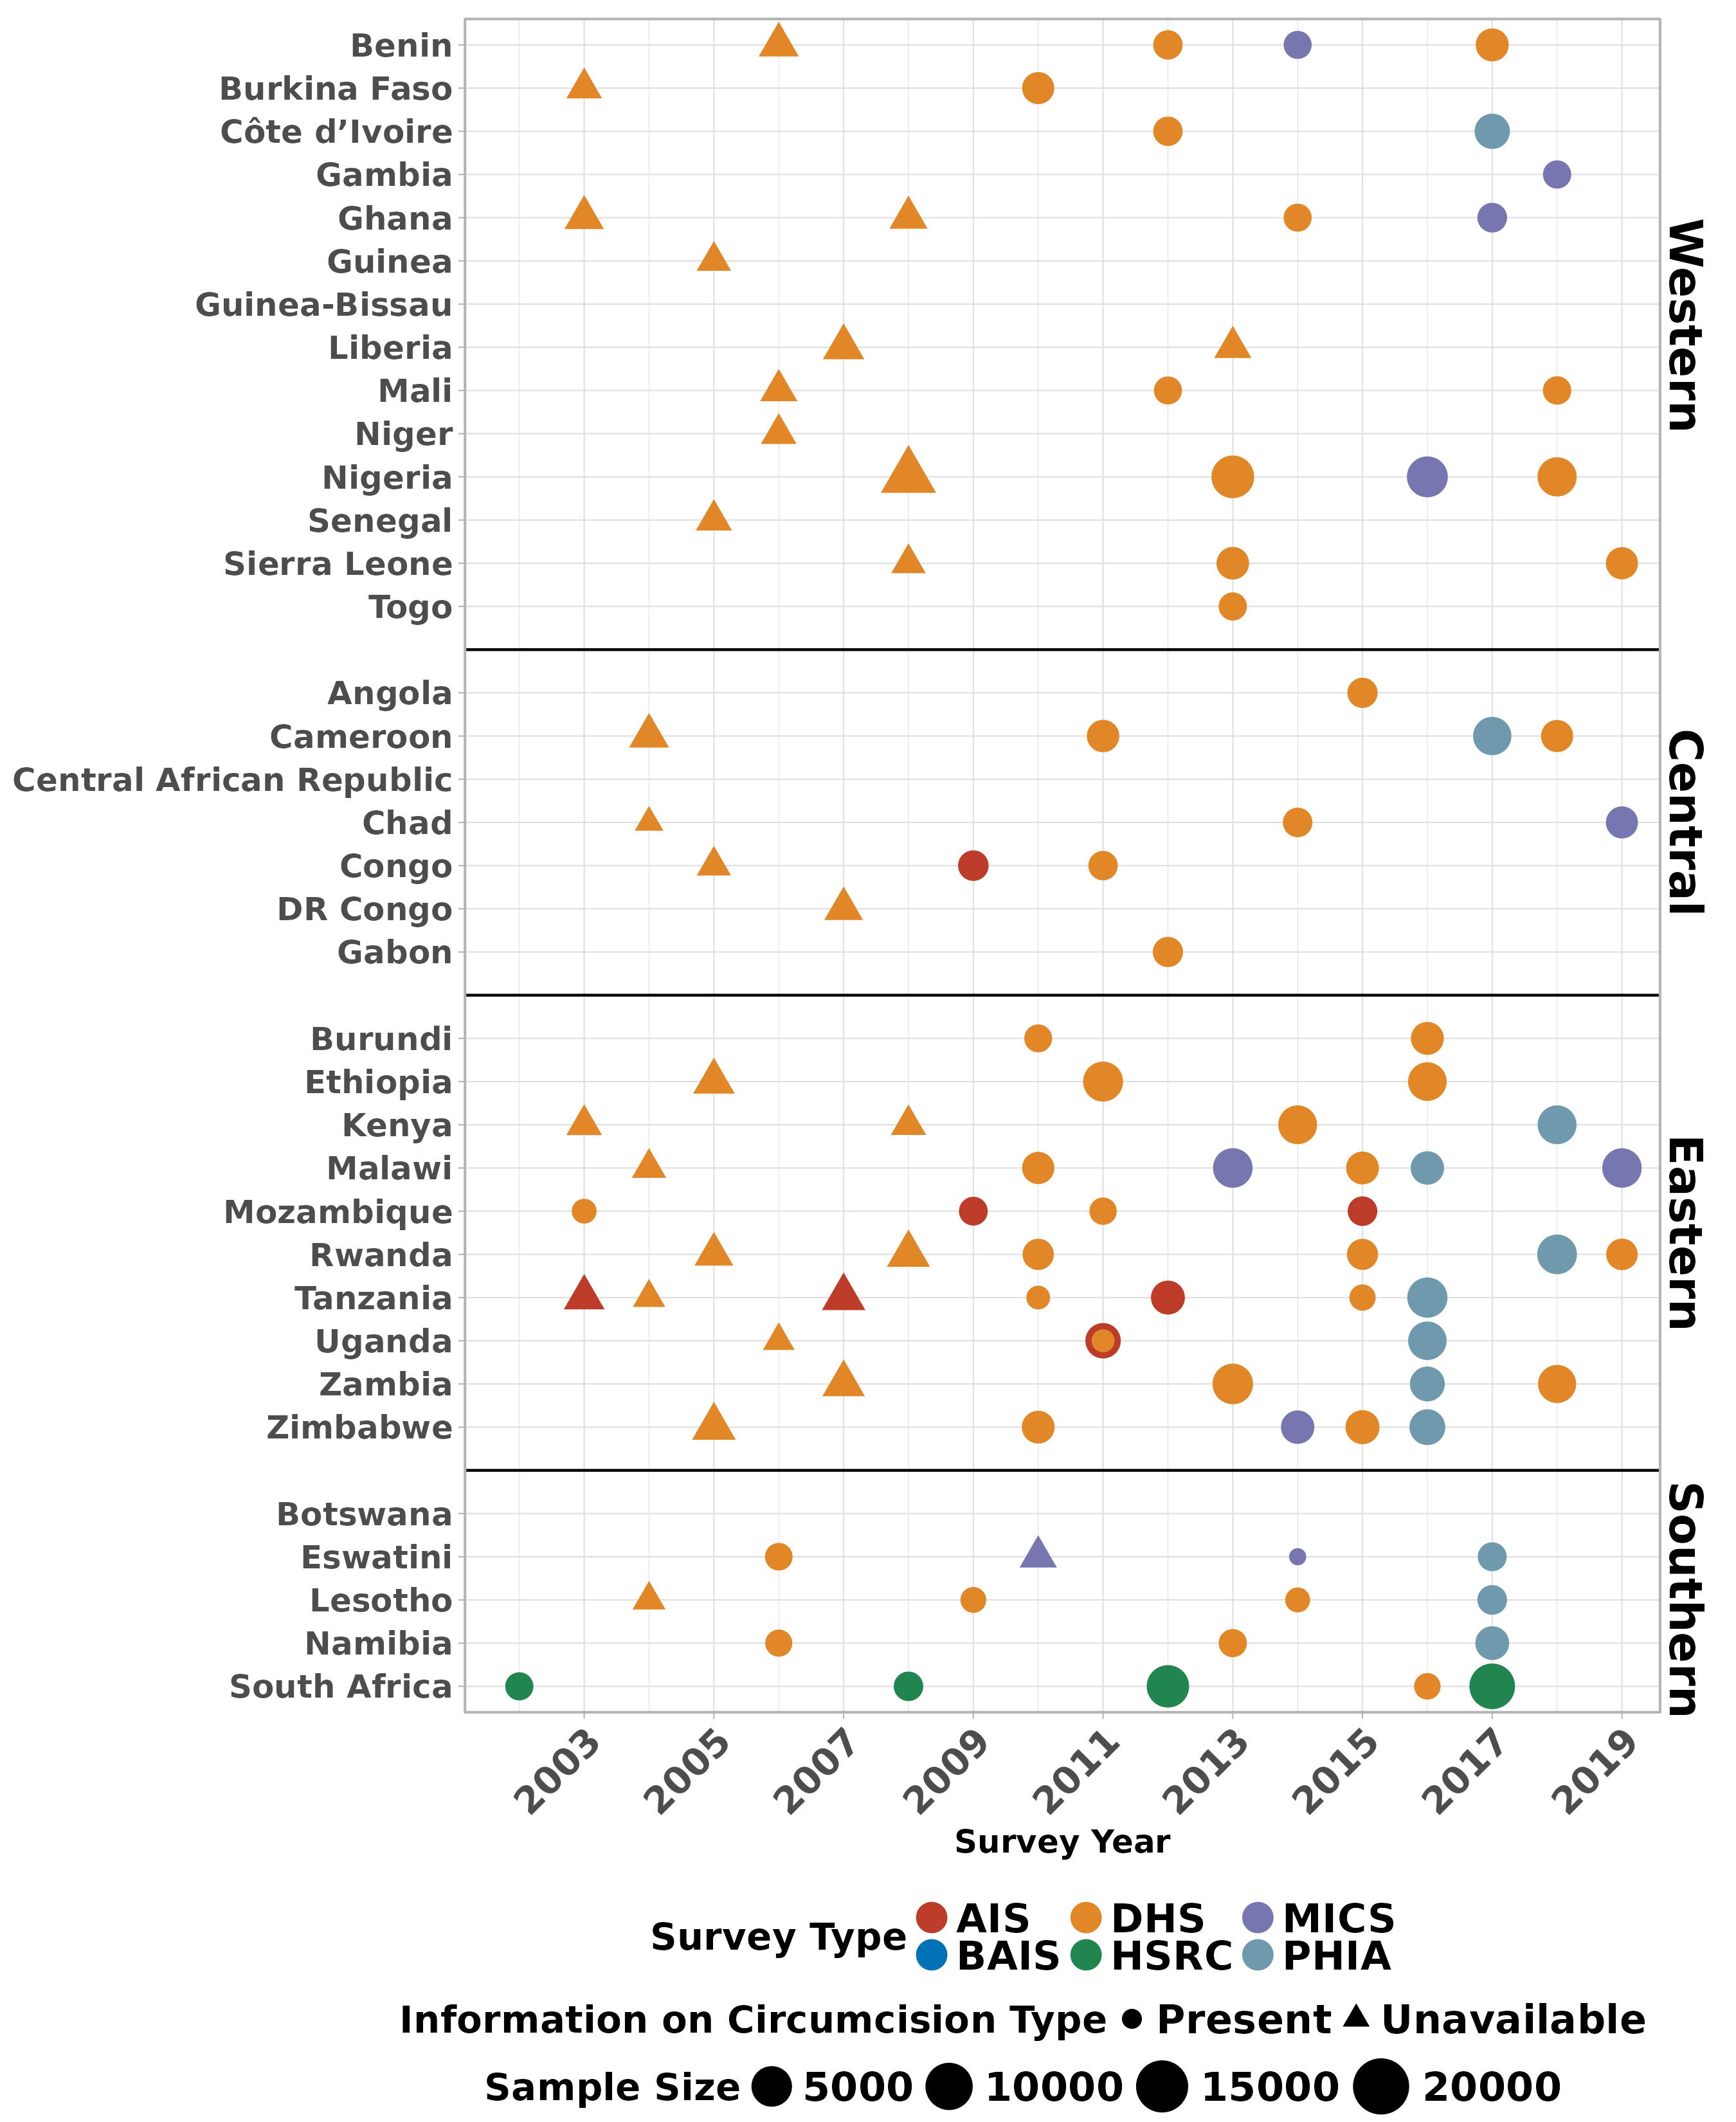
\includegraphics[width=.9\linewidth]{paper/plots/01_survey_table.png}
    \caption{Household surveys detailing circumcision patterns in sub-Saharan Africa. The colour and size of points are determined by the provider and sample size of each respective survey. Triangular points have no information on circumcision type.}
    \label{fig:enter-label}
\end{figure}

Demographic variables such as age, residence and survey sampling weight were extracted from all surveys, alongside information related to circumcision: self-reported circumcision status, age at circumcision, Who performed the circumcision (whether the individual was circumcised by a health worker/professional, traditional practioner, other or unknown) and Where did the circumcision take place (whether the individual was circumcised at a health facility, in the home of a health worker/professional, at home, at a ritual site, other or unknown). \textbf{[Write and link in survey table].}

% \begin{landscape}
{\linespread{1}
  \footnotesize 
\begin{longtable}[c]{ll ccc c}
      %%%%%%%%%%%%%%%%%%%%
      %%% Table header %%%
      %%%%%%%%%%%%%%%%%%%%
      % Upper layer of table header
      \hline
      % Lines inside the header
      \multicolumn{1}{l}{} & &  &  & \multicolumn{2}{c}{\bf Circumcision Type} \\ 
      \cmidrule(lr){5-6}
       & & {\bf Circumcision} & {\bf Age at} & {\bf Who performed} & {\bf Where was the}  \\
       & & {\bf Status} & {\bf Circumcision} & {\bf the circumcision?} & {\bf circumcision performed?} \\[5pt]
      % Lower lines
      \hline
      \vspace{-3pt}
      \endhead
      %%%%%%%%%%%%%%%%%%%%
      %%% Table footer %%%
      %%%%%%%%%%%%%%%%%%%%
      \\[-3pt] \hline
      \caption{Table of circumcision-related questions included in each survey for each sub-Saharan African country. Surveys which did not include a "Circumcision Status" and "Age at Circumcision" question could not be used, while circumcision type could not be inferred from surveys which did not have a "Who performed the circumcision" and/or "Where was the circumcision performed" question.}
      \endfoot
      %%%%%%%%%%%%%%%%%%%%%%
      %%% Table contents %%%
      %%%%%%%%%%%%%%%%%%%%%%
      \multicolumn{2}{l}{\textbf{Angola}} \\ 
& 2015 (DHS) & \checkmark & \checkmark & \checkmark & \checkmark \\[3pt] 
\multicolumn{2}{l}{\textbf{Benin}} \\ 
& 2006 (DHS) & \checkmark & \xmark & \xmark & \xmark \\ 
& 2012 (DHS) & \checkmark & \checkmark & \checkmark & \checkmark \\ 
& 2014 (MICS) & \checkmark & \checkmark & \checkmark & \checkmark \\ 
& 2017 (DHS) & \checkmark & \checkmark & \checkmark & \checkmark \\[3pt] 
\multicolumn{2}{l}{\textbf{Botswana}} \\ 
& 2008 (BAIS) & \checkmark & \xmark & \xmark & \checkmark \\ 
& 2013 (BAIS) & \checkmark & \xmark & \xmark & \checkmark \\[3pt] 
\multicolumn{2}{l}{\textbf{Burkina Faso}} \\ 
& 2003 (DHS) & \checkmark & \checkmark & \xmark & \xmark \\ 
& 2010 (DHS) & \checkmark & \checkmark & \checkmark & \checkmark \\[3pt] 
\multicolumn{2}{l}{\textbf{Burundi}} \\ 
& 2010 (DHS) & \checkmark & \checkmark & \checkmark & \checkmark \\ 
& 2016 (DHS) & \checkmark & \checkmark & \checkmark & \checkmark \\[3pt] 
\multicolumn{2}{l}{\textbf{Cameroon}} \\ 
& 2004 (DHS) & \checkmark & \xmark & \xmark & \xmark \\ 
& 2011 (DHS) & \checkmark & \checkmark & \checkmark & \checkmark \\ 
& 2017 (PHIA) & \checkmark & \checkmark & \checkmark & \xmark \\ 
& 2018 (DHS) & \checkmark & \checkmark & \checkmark & \checkmark \\[3pt] 
\multicolumn{2}{l}{\textbf{Central African Republic}} \\ 
& 2018 (MICS) & \checkmark & \checkmark & \checkmark & \checkmark \\[3pt] 
\multicolumn{2}{l}{\textbf{Chad}} \\ 
& 2004 (DHS) & \checkmark & \xmark & \xmark & \xmark \\ 
& 2014 (DHS) & \checkmark & \checkmark & \checkmark & \checkmark \\ 
& 2019 (MICS) & \checkmark & \checkmark & \checkmark & \checkmark \\[3pt] 
\multicolumn{2}{l}{\textbf{Congo - Kinshasa}} \\ 
& 2007 (DHS) & \checkmark & \xmark & \xmark & \xmark \\[3pt] 
\multicolumn{2}{l}{\textbf{Côte d’Ivoire}} \\ 
& 2012 (DHS) & \checkmark & \checkmark & \checkmark & \checkmark \\ 
& 2017 (PHIA) & \checkmark & \checkmark & \checkmark & \xmark \\[3pt] 
\multicolumn{2}{l}{\textbf{Eswatini}} \\ 
& 2006 (DHS) & \checkmark & \xmark & \checkmark & \xmark \\ 
& 2010 (MICS) & \checkmark & \checkmark & \xmark & \xmark \\ 
& 2014 (MICS) & \checkmark & \checkmark & \checkmark & \checkmark \\ 
& 2017 (PHIA) & \checkmark & \checkmark & \checkmark & \xmark \\[3pt] 
\multicolumn{2}{l}{\textbf{Ethiopia}} \\ 
& 2005 (DHS) & \checkmark & \xmark & \xmark & \xmark \\ 
& 2011 (DHS) & \checkmark & \checkmark & \checkmark & \checkmark \\ 
& 2016 (DHS) & \checkmark & \checkmark & \checkmark & \checkmark \\[3pt] 
\multicolumn{2}{l}{\textbf{Gabon}} \\ 
& 2012 (DHS) & \checkmark & \checkmark & \checkmark & \checkmark \\[3pt] 
\multicolumn{2}{l}{\textbf{Gambia}} \\ 
& 2018 (MICS) & \checkmark & \checkmark & \checkmark & \checkmark \\[3pt] 
\multicolumn{2}{l}{\textbf{Ghana}} \\ 
& 2003 (DHS) & \checkmark & \xmark & \xmark & \xmark \\ 
& 2008 (DHS) & \checkmark & \xmark & \xmark & \xmark \\ 
& 2014 (DHS) & \checkmark & \checkmark & \checkmark & \checkmark \\ 
& 2017 (MICS) & \checkmark & \checkmark & \checkmark & \checkmark \\[3pt] 
\multicolumn{2}{l}{\textbf{Guinea}} \\ 
& 2005 (DHS) & \checkmark & \xmark & \xmark & \xmark \\[3pt] 
\multicolumn{2}{l}{\textbf{Guinea-Bissau}} \\ 
& 2014 (MICS) & \checkmark & \checkmark & \checkmark & \checkmark \\ 
& 2018 (MICS) & \checkmark & \checkmark & \checkmark & \checkmark \\[3pt] 
\multicolumn{2}{l}{\textbf{Kenya}} \\ 
& 2003 (DHS) & \checkmark & \xmark & \xmark & \xmark \\ 
& 2008 (DHS) & \checkmark & \xmark & \xmark & \xmark \\ 
& 2014 (DHS) & \checkmark & \checkmark & \checkmark & \checkmark \\ 
& 2018 (PHIA) & \checkmark & \checkmark & \checkmark & \xmark \\[3pt] 
\multicolumn{2}{l}{\textbf{Lesotho}} \\ 
& 2004 (DHS) & \checkmark & \xmark & \xmark & \xmark \\ 
& 2009 (DHS) & \checkmark & \checkmark & \xmark & \checkmark \\ 
& 2014 (DHS) & \checkmark & \checkmark & \xmark & \checkmark \\ 
& 2017 (PHIA) & \checkmark & \checkmark & \checkmark & \xmark \\[3pt] 
\multicolumn{2}{l}{\textbf{Liberia}} \\ 
& 2007 (DHS) & \checkmark & \xmark & \xmark & \xmark \\ 
& 2013 (DHS) & \checkmark & \xmark & \xmark & \xmark \\[3pt] 
\multicolumn{2}{l}{\textbf{Malawi}} \\ 
& 2004 (DHS) & \checkmark & \xmark & \xmark & \xmark \\ 
& 2010 (DHS) & \checkmark & \checkmark & \checkmark & \checkmark \\ 
& 2013 (MICS) & \checkmark & \checkmark & \checkmark & \checkmark \\ 
& 2015 (DHS) & \checkmark & \checkmark & \checkmark & \checkmark \\ 
& 2016 (PHIA) & \checkmark & \checkmark & \checkmark & \xmark \\ 
& 2019 (MICS) & \checkmark & \checkmark & \checkmark & \checkmark \\[3pt] 
\multicolumn{2}{l}{\textbf{Mali}} \\ 
& 2006 (DHS) & \checkmark & \xmark & \xmark & \xmark \\ 
& 2012 (DHS) & \checkmark & \checkmark & \checkmark & \checkmark \\ 
& 2018 (DHS) & \checkmark & \checkmark & \checkmark & \checkmark \\[3pt] 
\multicolumn{2}{l}{\textbf{Mozambique}} \\ 
& 2003 (DHS) & \checkmark & \checkmark & \checkmark & \xmark \\ 
& 2009 (AIS) & \checkmark & \checkmark & \checkmark & \xmark \\ 
& 2011 (DHS) & \checkmark & \checkmark & \checkmark & \checkmark \\ 
& 2015 (AIS) & \checkmark & \checkmark & \checkmark & \checkmark \\[3pt] 
\multicolumn{2}{l}{\textbf{Namibia}} \\ 
& 2006 (DHS) & \checkmark & \xmark & \checkmark & \xmark \\ 
& 2013 (DHS) & \checkmark & \checkmark & \checkmark & \checkmark \\ 
& 2017 (PHIA) & \checkmark & \checkmark & \checkmark & \xmark \\[3pt] 
\multicolumn{2}{l}{\textbf{Niger}} \\ 
& 2006 (DHS) & \checkmark & \xmark & \xmark & \xmark \\[3pt] 
\multicolumn{2}{l}{\textbf{Nigeria}} \\ 
& 2008 (DHS) & \checkmark & \xmark & \xmark & \xmark \\ 
& 2013 (DHS) & \checkmark & \checkmark & \checkmark & \checkmark \\ 
& 2016 (MICS) & \checkmark & \checkmark & \checkmark & \checkmark \\ 
& 2018 (DHS) & \checkmark & \checkmark & \checkmark & \checkmark \\[3pt] 
\multicolumn{2}{l}{\textbf{Repulic of the Congo}} \\ 
& 2005 (DHS) & \checkmark & \xmark & \xmark & \xmark \\ 
& 2009 (AIS) & \checkmark & \xmark & \checkmark & \xmark \\ 
& 2011 (DHS) & \checkmark & \checkmark & \checkmark & \xmark \\[3pt] 
\multicolumn{2}{l}{\textbf{Rwanda}} \\ 
& 2005 (DHS) & \checkmark & \xmark & \xmark & \xmark \\ 
& 2008 (DHS) & \checkmark & \checkmark & \xmark & \xmark \\ 
& 2010 (DHS) & \checkmark & \checkmark & \checkmark & \checkmark \\ 
& 2015 (DHS) & \checkmark & \checkmark & \checkmark & \checkmark \\ 
& 2018 (PHIA) & \checkmark & \checkmark & \checkmark & \xmark \\ 
& 2019 (DHS) & \checkmark & \checkmark & \checkmark & \checkmark \\[3pt] 
\multicolumn{2}{l}{\textbf{Senegal}} \\ 
& 2005 (DHS) & \checkmark & \xmark & \xmark & \xmark \\[3pt] 
\multicolumn{2}{l}{\textbf{Sierra Leone}} \\ 
& 2008 (DHS) & \checkmark & \xmark & \xmark & \xmark \\ 
& 2013 (DHS) & \checkmark & \checkmark & \checkmark & \checkmark \\ 
& 2019 (DHS) & \checkmark & \checkmark & \checkmark & \checkmark \\[3pt] 
\multicolumn{2}{l}{\textbf{South Africa}} \\ 
& 2002 (HSRC) & \checkmark & \checkmark & \xmark & \checkmark \\ 
& 2008 (HSRC) & \checkmark & \checkmark & \checkmark & \checkmark \\ 
& 2012 (HSRC) & \checkmark & \checkmark & \checkmark & \checkmark \\ 
& 2016 (DHS) & \checkmark & \checkmark & \checkmark & \xmark \\ 
& 2017 (HSRC) & \checkmark & \checkmark & \checkmark & \checkmark \\[3pt] 
\multicolumn{2}{l}{\textbf{Tanzania}} \\ 
& 2003 (AIS) & \checkmark & \xmark & \xmark & \xmark \\ 
& 2004 (DHS) & \checkmark & \xmark & \xmark & \xmark \\ 
& 2007 (AIS) & \checkmark & \xmark & \xmark & \xmark \\ 
& 2010 (DHS) & \checkmark & \checkmark & \checkmark & \checkmark \\ 
& 2012 (AIS) & \checkmark & \checkmark & \checkmark & \checkmark \\ 
& 2015 (DHS) & \checkmark & \checkmark & \checkmark & \checkmark \\ 
& 2016 (PHIA) & \checkmark & \checkmark & \checkmark & \xmark \\[3pt] 
\multicolumn{2}{l}{\textbf{Togo}} \\ 
& 2013 (DHS) & \checkmark & \checkmark & \checkmark & \checkmark \\[3pt] 
\multicolumn{2}{l}{\textbf{Uganda}} \\ 
& 2006 (DHS) & \checkmark & \xmark & \xmark & \xmark \\ 
& 2011 (AIS) & \checkmark & \checkmark & \xmark & \checkmark \\ 
& 2011 (DHS) & \checkmark & \checkmark & \checkmark & \checkmark \\ 
& 2016 (DHS) & \checkmark & \checkmark & \checkmark & \checkmark \\ 
& 2016 (PHIA) & \checkmark & \checkmark & \checkmark & \xmark \\[3pt] 
\multicolumn{2}{l}{\textbf{Zambia}} \\ 
& 2007 (DHS) & \checkmark & \checkmark & \xmark & \xmark \\ 
& 2013 (DHS) & \checkmark & \checkmark & \checkmark & \checkmark \\ 
& 2016 (PHIA) & \checkmark & \checkmark & \checkmark & \xmark \\ 
& 2018 (DHS) & \checkmark & \checkmark & \checkmark & \checkmark \\[3pt] 
\multicolumn{2}{l}{\textbf{Zimbabwe}} \\ 
& 2005 (DHS) & \checkmark & \xmark & \xmark & \xmark \\ 
& 2010 (DHS) & \checkmark & \checkmark & \checkmark & \checkmark \\ 
& 2014 (MICS) & \checkmark & \checkmark & \checkmark & \checkmark \\ 
& 2015 (DHS) & \checkmark & \checkmark & \checkmark & \checkmark \\ 
& 2016 (PHIA) & \checkmark & \checkmark & \checkmark & \xmark 
\end{longtable}
}


\begin{landscape}
    {\linespread{1}
  \footnotesize 
\begin{longtable}[c]{ll cccc ccc ccc}
      %%%%%%%%%%%%%%%%%%%%
      %%% Table header %%%
      %%%%%%%%%%%%%%%%%%%%
      % Upper layer of table header
      \hline
      % Lines inside the header
      \multicolumn{1}{l}{} & & \multicolumn{4}{c}{\bf Survey questions} & \multicolumn{2}{c}{\bf Sample size} & \multicolumn{2}{c}{\bf Circumcision status} & \multicolumn{2}{c}{\bf Circumcision metadata} \\
      \cmidrule(lr){3-6} \cmidrule(lr){7-8}\cmidrule(lr){9-10} \cmidrule(lr){11-12}
       & & {\bf Circ.} & {\bf Age at} & {\bf Who} & {\bf Where } & \multirow{2}{*}{\bf Total} & \multirow{2}{*}{\bf Included (\%)} & \multirow{2}{*}{\bf Uncircumcised (\%)} & \multirow{2}{*}{\bf Circumcised (\%)} & {\bf Known age} & {\bf Known type}
       \\
       & & {\bf Status} & {\bf Circ.} & {\bf performed?} & {\bf performed?}  & & & & & {\bf at circ. (\%)} & {\bf of circ. (\%)} \\[5pt]
      % Lower lines
      \hline
      \vspace{-3pt}
      \endhead
      %%%%%%%%%%%%%%%%%%%%
      %%% Table footer %%%
      %%%%%%%%%%%%%%%%%%%%
      \\[-3pt] \hline
      \endfoot
      %%%%%%%%%%%%%%%%%%%%%%
      %%% Table contents %%%
      %%%%%%%%%%%%%%%%%%%%%%
      \multicolumn{2}{l}{\textbf{Angola}} \\ 
& 2015 (DHS) & \checkmark & \checkmark & \checkmark & \checkmark & 5684 & 5660 (99.58\%) & 207 (3.66\%) & 5453 (96.34\%) & 4106 (75.30\%) & 4767 (75.30\%) \\[3pt]
\multicolumn{2}{l}{\textbf{Benin}} \\ 
& 2006 (DHS) & \checkmark & \xmark & \xmark & \xmark & 5321 & 5317 (99.92\%) & 234 (4.40\%) & 5083 (95.60\%) & 0 (0.00\%) & 0 (0.00\%) \\ 
& 2012 (DHS) & \checkmark & \checkmark & \checkmark & \checkmark & 5153 & 5129 (99.53\%) & 354 (6.90\%) & 4775 (93.10\%) & 2709 (56.73\%) & 4328 (56.73\%) \\  
& 2014 (MICS) & \checkmark & \checkmark & \checkmark & \checkmark & 4577 & 4370 (95.48\%) & 124 (2.84\%) & 4246 (97.16\%) & 4141 (97.53\%) & 4210 (97.53\%) \\  
& 2017 (DHS) & \checkmark & \checkmark & \checkmark & \checkmark & 7595 & 7569 (99.66\%) & 401 (5.30\%) & 7168 (94.70\%) & 2514 (35.07\%) & 7063 (35.07\%) \\[3pt]
\end{longtable}

\begin{longtable}[c]{ll ccc ccc}
      %%%%%%%%%%%%%%%%%%%%
      %%% Table header %%%
      %%%%%%%%%%%%%%%%%%%%
      % Upper layer of table header
      \hline
      % Lines inside the header
      \multicolumn{1}{l}{} & & \multicolumn{2}{c}{\bf Sample size} & \multicolumn{2}{c}{\bf Circumcision status} & \multicolumn{2}{c}{\bf Circumcision metadata} \\ 
      \cmidrule(lr){3-4} \cmidrule(lr){5-6}\cmidrule(lr){7-8} 
       & & \multirow{2}{*}{\bf Total} & \multirow{2}{*}{\bf Included (\%)} & \multirow{2}{*}{\bf Uncircumcised (\%)} & \multirow{2}{*}{\bf Circumcised (\%)} & {\bf Known age at} & {\bf Known type of}
       \\
       & & & & & & {\bf circumcision (\%)} & {\bf circumcision (\%)} \\[5pt]
      % Lower lines
      \hline
      \vspace{-3pt}
      \endhead
      %%%%%%%%%%%%%%%%%%%%
      %%% Table footer %%%
      %%%%%%%%%%%%%%%%%%%%
      \\[-3pt] \hline
      \endfoot
      %%%%%%%%%%%%%%%%%%%%%%
      %%% Table contents %%%
      %%%%%%%%%%%%%%%%%%%%%%
\multicolumn{2}{l}{\textbf{Angola}} \\ 
& 2015 (DHS) & 5684 & 5660 (99.58\%) & 207 (3.66\%) & 5453 (96.34\%) & 4106 (75.30\%) & 4767 (75.30\%) \\[3pt]
\multicolumn{2}{l}{\textbf{Benin}} \\ 
& 2006 (DHS) & 5321 & 5317 (99.92\%) & 234 (4.40\%) & 5083 (95.60\%) & 0 (0.00\%) & 0 (0.00\%) \\ 
& 2012 (DHS) & 5153 & 5129 (99.53\%) & 354 (6.90\%) & 4775 (93.10\%) & 2709 (56.73\%) & 4328 (56.73\%) \\ 
& 2014 (MICS) & 4577 & 4370 (95.48\%) & 124 (2.84\%) & 4246 (97.16\%) & 4141 (97.53\%) & 4210 (97.53\%) \\ 
& 2017 (DHS) & 7595 & 7569 (99.66\%) & 401 (5.30\%) & 7168 (94.70\%) & 2514 (35.07\%) & 7063 (35.07\%) \\[3pt]
\end{longtable}
}
\end{landscape}








  




The age of respondents was calculated from the century-month-code (CMC) of birth and interview dates. 
Survey respondents were located to their districts using masked cluster geocoordinates. 
Where these coordinates were unavailable (as in several MICS surveys) respondents were located to their level 1 administrative boundaries, most often corresponding to a province.  

Circumcisions were classed as a medical male circumcision (MMC) or traditional male circumcision (TMC) based on how responses to both ‘Who performed the circumcision?’ and ‘Where did the circumcision take place?’ were classified \textbf{[Link to the table]}. 
Respondents that did not have any information related to the type of circumcision were classified as having “unknown” male circumcision (MC) type.   

{\linespread{1}
\begin{table}[htbp]
	\centering
    \footnotesize
	\caption{Criteria used to classify circumcisions from the survey data as MMC or TMC.}
	\label{tab::MCclassification}
	\begin{tabular}{c l | c c c}
	\multirow{2}{*}{} & & \multicolumn{3}{c}{\bf Who performed the circumcision?} \\
	                    &      & \begin{tabular}{c}\bf Healthcare\\[-5pt] \bf Professional\end{tabular} & \begin{tabular}{c}\bf Traditional \\[-5pt] \bf Practioner\end{tabular} & \begin{tabular}{c}\bf Missing\end{tabular} \\
	                          \hline
		% \multirow{3}{*}{\rotatebox{90}{Where performed?}}  & \begin{tabular}{l}Healthcare Facility\end{tabular} & MMC & MMC & MMC \\
		\multirow{3}{*}{\rotatebox{90}{\begin{tabular}{c}\bf Where was it\\[-5pt] \bf performed?\end{tabular}}}  & \begin{tabular}{l}\bf Healthcare\\[-5pt] \bf Facility \end{tabular} & MMC & MMC & MMC \\
		& \begin{tabular}{l}\bf Home, School \\[-5pt] \bf or Ritual Site \end{tabular} & MMC & TMC & TMC \\
		& \begin{tabular}{l} \bf Missing\end{tabular} & MMC & TMC & MC \\
	\end{tabular}	
\end{table}
}

In total, information was extracted from XXX, XXX respondents from all surveys.
\textbf{[Participation rates table]}
\todo{Get Matt to make dummy table for me based on this info for 2-3 countries, then I can fill in}



















%%%%%%%%%%%%%%%%%%%%%%%%%%%%%%%%%%%%%%%%%%%%%%%%%%%%%%%%%%%%%%%%%%
%%%%%%%%%%%%%%%%%%%%%%%%%%%%%%%%%%%%%%%%%%%%%%%%%%%%%%%%%%%%%%%%%%

\subsection{Administrative boundaries}
\label{sec:org0995c95}

%%%%%%%%%%%%%%%%%%%%%%%%%%%%%%%%%%%%%%%%%%%%%%%%%%%%%%%%%%%%%%%%%%
%%%%%%%%%%%%%%%%%%%%%%%%%%%%%%%%%%%%%%%%%%%%%%%%%%%%%%%%%%%%%%%%%%

[Add in information about the boundaries] 
\todo{Section for Jeff}

%%%%%%%%%%%%%%%%%%%%%%%%%%%%%%%%%%%%%%%%%%%%%%%%%%%%%%%%%%%%%%%%%%
%%%%%%%%%%%%%%%%%%%%%%%%%%%%%%%%%%%%%%%%%%%%%%%%%%%%%%%%%%%%%%%%%%

\subsection{Population}
\label{sec:org0d7d6e9}

%%%%%%%%%%%%%%%%%%%%%%%%%%%%%%%%%%%%%%%%%%%%%%%%%%%%%%%%%%%%%%%%%%
%%%%%%%%%%%%%%%%%%%%%%%%%%%%%%%%%%%%%%%%%%%%%%%%%%%%%%%%%%%%%%%%%%

Estimates for the male population size by district and five-year age group from 2002 through 2019 were sourced from XXX. 
Distributed (?) to single-year of age according to ??? 
\todo{Section for Jeff}

%%%%%%%%%%%%%%%%%%%%%%%%%%%%%%%%%%%%%%%%%%%%%%%%%%%%%%%%%%%%%%%%%%
%%%%%%%%%%%%%%%%%%%%%%%%%%%%%%%%%%%%%%%%%%%%%%%%%%%%%%%%%%%%%%%%%%
%%%%%%%%%%%%%%%%%%%%%%%%%%%%%%%%%%%%%%%%%%%%%%%%%%%%%%%%%%%%%%%%%%

\section{Model}
\label{sec:org38d457a}

%%%%%%%%%%%%%%%%%%%%%%%%%%%%%%%%%%%%%%%%%%%%%%%%%%%%%%%%%%%%%%%%%%
%%%%%%%%%%%%%%%%%%%%%%%%%%%%%%%%%%%%%%%%%%%%%%%%%%%%%%%%%%%%%%%%%%
%%%%%%%%%%%%%%%%%%%%%%%%%%%%%%%%%%%%%%%%%%%%%%%%%%%%%%%%%%%%%%%%%%

{\color{red} \bf
To do:
\begin{itemize}
    \item Model calibration
    \item Prior choice
    \item Citations
\end{itemize}}

Following a similar approach to \cite{thomas2021multilevel}, we developed a Bayesian hierarchical model with small area estimation methods that uses survey data to estimate the probabilities and coverage of circumcision using a competing risk discrete time-to-event model stratified by region, age, time, and type. We modelled each country independently rather than a model by sub-region or for the whole of sub-Saharan due to computational constraints and we modelled probabilities of circumcision at the organizational level in which the country team has prioritised their program, called the PSNU area level, or the most granular level available in surveys (hereafter called the district-level). 

In countries where suitable survey information was collected on circumcision type, we consider the following two types of circumcision: (1) circumcisions that occurred in traditional male initiation ceremonies or for other religious or cultural reasons (TMC) and (2) circumcisions for non-traditional reasons and/or HIV prevention that take place in a clinical setting using medical methods (MMC). Some countries did not have any surveys that collected information on the type of circumcision (see above), so we were unable to conduct an analysis of the probabilities of circumcision by type. For these countries, we consider estimating the probability and coverage of circumcision of any or (unknown) type (MC) only. 

%%%%%%%%%%%%%%%%%%%%%%%%%%%%%%%%%%%%%%%%%%%%%%%%%%%%%%%%%%%%%%%%%%
%%%%%%%%%%%%%%%%%%%%%%%%%%%%%%%%%%%%%%%%%%%%%%%%%%%%%%%%%%%%%%%%%%

\subsection{Probabilities of circumcision (by type)}
\label{sec::bytype}

%%%%%%%%%%%%%%%%%%%%%%%%%%%%%%%%%%%%%%%%%%%%%%%%%%%%%%%%%%%%%%%%%%
%%%%%%%%%%%%%%%%%%%%%%%%%%%%%%%%%%%%%%%%%%%%%%%%%%%%%%%%%%%%%%%%%%

In countries where suitable survey information was collected on circumcision type, we used survey data to model the probabilities of receiving a TMC, MMC or MC for individuals residing in district $i \in I = \{1, 2, \ldots, N_I\}$ at age $a \in A = \{0, 1, 2, \ldots, N_A\}$ and time $t \in T = \{1, 2, \ldots, N_T\}$. 

%%%%%%%%%%%%%%%%%%%%%%%%%%%%%%%%%%%%%%%%%%%%%%%%%%%%%%%%%%%%%%%%%%

\subsubsection*{Traditional circumcision}

%%%%%%%%%%%%%%%%%%%%%%%%%%%%%%%%%%%%%%%%%%%%%%%%%%%%%%%%%%%%%%%%%%

\noindent We define $\lambda^{\text{TMC}}_{iat}$ as the probability that an individual in district $i$ received TMC at age $a$ and time step $t$, given they were uncircumcised by age $a-1$ and time $t-1$, 
\begin{equation} 
		\lambda^{\text{TMC}}_{iat} = \mathbb{P}(\text{TMC} \; \text{in} \; (i,a,t) \; | \; \text{Uncircumcised in} \; (i,a-1, t-1)). 
	\label{eqn::TMC}
\end{equation}
A key assumption of the \cite{thomas2021multilevel} model was that TMC was constant over time, due to traditional male initiation ceremonies amongst tribal, cultural and religious groups remained stable over time in South Africa however an assumption of a constant probability of TMC might not be feasible everywhere. For example, in some countries the level and practices of TMC have changed through time due to demographic shifts. There has also been a replacement of TMCs through MMCs observed, particularly in VMMC priority countries, to ensure HIV prevention efficacy and/or for safety considerations \cite{thomas2021multilevel}. Furthermore, there may also be cases where TMC remains stable and allowing a constant probability of TMC in the competing risks framework will cause a reduction in TMC coverage overall in places where VMMC uptake is high. Here, we consider two models for $\lambda^{\text{TMC}}_{iat}$ in each country: (i) time invariant (i.e. constant over time) and (ii) time variant (i.e. varying over time). 

The {\it time-invariant} probability of TMC was modelled using a piece-wise logit-linear function, 
\begin{equation*} 
	\text{logit}(\lambda^{\text{TMC}}_{iat}) = \hat{\alpha} + \hat{\psi}_i + \hat{\phi}_a + \hat{\gamma}_{ia}
\end{equation*}
where $\hat{\alpha}$ is the intercept, $\hat{\psi_i}$ is a district random effect, $\hat{\phi}_a$ is an age random effect, and $\hat{\gamma}_{ia}$ is an age-district interaction term to allow different age patterns of TMC across districts. The {\it time-variant} probability of TMC was also modelled using a piece-wise logit-linear function, 
\begin{equation*} 
	\text{logit}(\lambda^{\text{TMC}}_{iat}) = \hat{\alpha} + \hat{\psi}_i + \hat{\phi}_a + \hat{\theta}_t + \hat{\gamma}_{ia} + \hat{\delta}_{at}
\end{equation*}
where $\hat{\alpha}$ is the intercept, $\hat{\psi_i}$ is a district random effect, $\hat{\phi}_a$ is an age random effect, $\theta_i$ is a temporal random effect,  $\hat{\gamma}_{ia}$ is an age-district interaction term to allow different age patterns of TMC across districts and $\hat{\delta}_{at}$ is an age-time interaction term to allow for different age patterns of TMCs over time. We did not include a district-time interaction into due to computational constraints. 

Whether a country used a time-invariant or time-variant probability of TMC was chosen depending on which produced the best within-sample model fit (see Section \ref{sec::modelcheck} for further details). 

%%%%%%%%%%%%%%%%%%%%%%%%%%%%%%%%%%%%%%%%%%%%%%%%%%%%%%%%%%%%%%%%%%

\subsubsection*{Medical circumcision}

%%%%%%%%%%%%%%%%%%%%%%%%%%%%%%%%%%%%%%%%%%%%%%%%%%%%%%%%%%%%%%%%%%

\noindent We defined $\lambda^{\text{MMC}}_{iat}$ as the probability an individual in district $i$ received MMC at age $a$ and time $t$, given they were uncircumcised by age $a-1$ and time $t-1$,  
\begin{equation*}
		\lambda^{\text{MMC}}_{iat} = \mathbb{P}(\text{MMC} \; \text{in} \; (i,a,t) \; | \; \text{Uncircumcised in} \; (i,a-1, t-1)),
\end{equation*}
To ensure $\lambda^{\text{TMC}}_{iat} + \lambda^{\text{MMC}}_{iat} \leq 1$ for all $i$, $a$ and $t$ in the discrete-time framework, we assumed the TMC prior to MMC in each time step. Therefore, we condition on this and practically model the probability an individual in district $i$ received an MMC at age $a$ and time $t$, given they were uncircumcised by age $a-1$ and time $t-1$ and did not receive TMC at age $a$ and time $t$
\begin{equation*}
		\tilde{\lambda}^{\text{MMC}}_{iat} = \mathbb{P}(\text{MMC} \; \text{in} \; (i,a,t) \; | \; \text{Uncircumcised in} \; (i,a-1, t-1) \text{ and no TMC in} \; (i,a, t))
\end{equation*}
It then follows that 
\begin{equation*}
		\lambda^{\text{MMC}}_{iat} = \tilde{\lambda}^{\text{MMC}}_{iat}\cdot (1-\lambda^{\text{TMC}}_{iat}).
\end{equation*}

The provision of MMC is highly heterogeneous in sub-Saharan Africa and has changed substantially since 2008, particularly in countries that have programmes to scale-up MMC for HIV prevention. VMMC programmes provide MMCs for HIV prevention to those aged 10 and over, while infant and paediatric medical circumcision often occurs through cultural or religious practices unrelated to scale-up of VMMC for HIV prevention. Due to this, Thomas et al. \cite{thomas2021multilevel} separated the probability of MMC, $\tilde{\lambda}^{\text{MMC}}_{iat}$, into two processes: (i) paediatric circumcision (for those aged 0--9) and (ii) adolescent and adult circumcision (for those aged 10 and over). This ensured that any increase in MMC for those aged 10 and over did not bias the probability of MMC in those under 10 in South Africa. However, this may not be appropriate everywhere, particularly in countries without programmes to upscale MMC coverage. Therefore, we consider two models for $\lambda^{\text{MMC}}_{iat}$ in each country: (i) no cut-off and (ii) paediatric cut off.

We modelled the probability of MMC {\it with no cut-off} using a piece-wise logit-linear function, 
\begin{equation*}
	\text{logit}(\tilde{\lambda}^{\text{MMC}}_{iat}) = \alpha + \psi_i + \phi_a + \theta_t + \gamma_{ia} + \delta_{at} + \zeta_{it} 
\end{equation*}
where $\alpha$ is the intercept, $\psi_i$ is a district random effect, $\theta_i$ is a temporal random effect, $\phi_a$ is an age random effect, $\gamma_{ia}$ is an age-district interaction terms to allow for different patterns of MMCs over age between districts, $\delta_{at}$ is an age-time interaction term to account for any changing age patterns in MMCs over time and $\zeta_{it}$ is an district-time interaction term to allow for different uptake of MMCs over time across districts. We also modelled the probability of MMC {\it with a paediatric cut-off} using a piece-wise logit-linear function, 
\begin{equation*}
	\text{logit}(\tilde{\lambda}^{\text{MMC}}_{iat}) =
	\begin{cases}
		\bar{\alpha} + \bar{\psi}_i + \bar{\phi}_a + \bar{\gamma}_{ia} & \text{for } 0 \leq a \leq 9\\
		\alpha + \psi_i + \phi_a + \theta_t + \gamma_{ia} + \delta_{at} + \zeta_{it} & \text{for } a \geq 10
	\end{cases} 
\end{equation*}
where $\bar{\alpha}$ and $\alpha$ are intercepts, $\bar{\psi}_i$ and $\psi_i$ are district random effects, $\theta_i$ are temporal random effects, $\bar{\phi}_a$ and $\phi_a$ are age random effects, $\bar{\gamma}_{ia}$ and $\gamma_{ia}$ are age-district interaction terms for paediatric circumcision and adolescent and adult circumcision respectively. The $\delta_{at}$ is an age-time interaction term to allow for different age patterns of MMCs over time and $\zeta_{it}$ is an space-time interaction term to allow for different uptake of MMCs over time across districts in adolescent and adult men. We assume that the probability of MMC among those aged 0--9 were constant over time, (i.e. $\lambda^{\text{MMC}}_{iat} \equiv \lambda^{\text{MMC}}_{ia}$ when $0\leq a \leq 9$), as paediatric medical circumcision practices are unrelated to VMMC for HIV prevention and are relatively stable. 

The choice of whether a country used a paediatric cut-off or no cut-off in the probability of MMC was chosen depending on which produced the best within-sample model fit (see Section \ref{sec::modelcheck} for further details). 

%%%%%%%%%%%%%%%%%%%%%%%%%%%%%%%%%%%%%%%%%%%%%%%%%%%%%%%%%%%%%%%%%%

\subsubsection*{Circumcision of any (or unknown) type}

%%%%%%%%%%%%%%%%%%%%%%%%%%%%%%%%%%%%%%%%%%%%%%%%%%%%%%%%%%%%%%%%%%

\noindent We define $\lambda^{\text{MC}}_{iat}$ as the probability of circumcision of any (or unknown) type, at age $a$ and time $t$ given they were uncircumcised by age $a-1$ and time $t-1$ 
\begin{equation*}
	\lambda^{\text{MC}}_{iat} = \mathbb{P}(\text{MC} \; \text{in} \; (i,a,t) \; | \; \text{Uncircumcised in} \; (i,a-1,t-1))
\end{equation*}
and this is modelled using the sum of having either a TMC or MMC at age $a$ and time $t$ given they were uncircumcised by age $a-1$ and time $t-1$,
\begin{equation*}
	\lambda^{\text{MC}}_{iat} = \lambda^{\text{TMC}}_{ia} + \lambda^{\text{MMC}}_{iat}. 
\end{equation*}

%%%%%%%%%%%%%%%%%%%%%%%%%%%%%%%%%%%%%%%%%%%%%%%%%%%%%%%%%%%%%%%%%%
%%%%%%%%%%%%%%%%%%%%%%%%%%%%%%%%%%%%%%%%%%%%%%%%%%%%%%%%%%%%%%%%%%

\subsection{Probabilities of circumcision (typeless)}
\label{sec::typeless}

%%%%%%%%%%%%%%%%%%%%%%%%%%%%%%%%%%%%%%%%%%%%%%%%%%%%%%%%%%%%%%%%%%
%%%%%%%%%%%%%%%%%%%%%%%%%%%%%%%%%%%%%%%%%%%%%%%%%%%%%%%%%%%%%%%%%%

In countries that did not have a survey that contained information on the type of circumcision, we used survey data to model the probabilities of receiving a MC of any (or unknown) type for individuals residing in district $i \in I = \{1, 2, \ldots, N_I\}$ at age $a \in A = \{0, 1, 2, \ldots, N_A\}$ and time $t \in T = \{1, 2, \ldots, N_T\}$. 

\noindent We define $\lambda^{\text{MC}}_{iat}$ as the probability that an individual in district $i$ received a circumcision (either a TMC or MMC) at age $a$ and time step $t$, given they were uncircumcised by age $a-1$ and time $t-1$, 
\begin{equation} 
		\lambda^{\text{MC}}_{iat} = \mathbb{P}(\text{MC} \; \text{in} \; (i,a,t) \; | \; \text{Uncircumcised in} \; (i,a-1, t-1)). 
	\label{eqn::MC}
\end{equation}
We modelled the probability of MC using a piece-wise logit-linear function:
\begin{equation*}
	\text{logit}(\lambda^{\text{MC}}_{iat}) = \alpha + \psi_i + \phi_a + \theta_t + \gamma_{ia} + \delta_{at} + \zeta_{it} 
\end{equation*}
where $\alpha$ is the intercept, $\psi_i$ is a district random effect, $\theta_i$ is a temporal random effect, $\phi_a$ is an age random effect, $\gamma_{ia}$ is an age-district interaction terms to allow for different patterns of MCs over age between districts, $\delta_{at}$ is an age-time interaction term to account for any changing age patterns in MCs over time and $\zeta_{it}$ is an district-time interaction term to allow for different uptake of MCs over time across districts. 

%%%%%%%%%%%%%%%%%%%%%%%%%%%%%%%%%%%%%%%%%%%%%%%%%%%%%%%%%%%%%%%%%%
%%%%%%%%%%%%%%%%%%%%%%%%%%%%%%%%%%%%%%%%%%%%%%%%%%%%%%%%%%%%%%%%%%

\subsection{Circumcision coverage}
\label{sec::coverage}

%%%%%%%%%%%%%%%%%%%%%%%%%%%%%%%%%%%%%%%%%%%%%%%%%%%%%%%%%%%%%%%%%%
%%%%%%%%%%%%%%%%%%%%%%%%%%%%%%%%%%%%%%%%%%%%%%%%%%%%%%%%%%%%%%%%%%

We define the probability of remaining uncircumcised, $S_{iat}$, in district $i$, at age $a$ and time $t$ (often called the survivor function), is estimated using, 
\begin{equation*}
	\begin{split}
		S_{iat} &= \mathbb{P}(\text{Uncircumcised in} \; (i,a-1,t-1)) \\
				&= \prod_{(0,(t-a))}^{(a-1,t-1)}\lambda^{\text{UC}}_{iat} \\
				&= \lambda^{\text{UC}}_{i,0,t-a}\cdot \lambda^{\text{UC}}_{i,1,t-a+1}\cdot\ldots \cdot\lambda^{\text{UC}}_{i,a-1,t-1}
	\end{split}
	\label{eqn::survfunc}
\end{equation*}
where $\lambda^{\text{UC}}_{iat}$ is the probability an individual in district $i$ remained uncircumcised at age $a$ and time $t$, given they were uncircumcised by age $a-1$ and time $t-1$,
\begin{equation*}
	\begin{split}
		\lambda^{\text{UC}}_{iat} &= \mathbb{P}(\text{Uncircumcised in}  \; (i,a,t) \; | \; \text{Uncircumcised in} \; (i,a-1, t-1)),\\
		&= 1 - \lambda^{\text{MC}}_{iat} 
	\end{split}
	\label{eqn::uncirc}
\end{equation*}

The cumulative incidence function (CIF) defines the marginal probability (or coverage/proportion) of individuals residing in district $i$ who received a TMC, MMC or MC of any (or unknown) type by age $a$ and time $t$, accounting for the competing risk of other circumcision types. This was calculated as the sum of incidence of circumcision by type $k$ at each age up to $a$:
\begin{equation*}
	\begin{split}
		\text{CIF}_{iat}^k &= \mathbb{P}(k \; \text{by} \; (i,a,t)) \\
		&= \sum_{(0,(t-a))}^{(a,t)} I^k_{iat}
	\end{split}
	\label{eqn::cuminc}
\end{equation*}
where $I^k_{iat}$ is the incidence of circumcision of type $k\in \{\textrm{TMC}, \textrm{MMC}, \textrm{MC}\}$, in region $i$, at age $a$ and time $t$, 
\begin{equation*}
	\begin{split}
		I_{iat}^k &= \mathbb{P}(k \; \text{in} \; (i,a,t)) \\
		       &= \mathbb{P}(k \; \text{in} \; (i,a,t) | \; \text{Uncircumcised in} \; (i,a-1,t-1))\times \\
		       & \;\;\;\;\;\;\;\;\;\;\;\;\;\;\;\;\;\mathbb{P}(\text{Uncircumcised in} \; (i,a-1,t-1)) \\
	    	   &= \lambda_{iat}^k \cdot S_{iat} 
	\end{split}
	\label{eqn::inc}
\end{equation*}

%%%%%%%%%%%%%%%%%%%%%%%%%%%%%%%%%%%%%%%%%%%%%%%%%%%%%%%%%%%%%%%%%%
%%%%%%%%%%%%%%%%%%%%%%%%%%%%%%%%%%%%%%%%%%%%%%%%%%%%%%%%%%%%%%%%%%

\subsection{Model priors}
\label{sec::priors}

%%%%%%%%%%%%%%%%%%%%%%%%%%%%%%%%%%%%%%%%%%%%%%%%%%%%%%%%%%%%%%%%%%
%%%%%%%%%%%%%%%%%%%%%%%%%%%%%%%%%%%%%%%%%%%%%%%%%%%%%%%%%%%%%%%%%%

In space, we assigned the random effects $\hat{\psi}_i$, $\bar{\psi}_i$, $\psi_i$, $\hat{\gamma}_{ia}$, $\gamma_{ia}$ and $\zeta_{it}$, intrinsic conditional autoregressive (ICAR) priors \cite{besag1995conditional}. An ICAR model allows us to encode spatial dependence between neighbouring regions which allows information on the probability and coverage of circumcision in areas where data is sparse or non-existent to be borrowed. For a generic parameter $\beta_i$, an ICAR model assumes that the mean of $\beta_i$ is a weighted average its neighbours, 
\begin{equation*}
	\beta_i \;|\; \beta_{j}, j \sim i, \tau_{\beta} \sim \text{N}\left(\frac{1}{n_i} \sum_{j \sim i} \beta_j, \frac{1}{n_i\tau_{\beta}} \right) \;\;\; i = 1, 2, 3,\ldots, N_I
\end{equation*}
Here, $j \sim i$ refers to the neighbours of region $i$, $n_i$ is the number of neighbours and $\tau_{\beta}$ is the marginal precision \cite{rue2005gaussian}. The joint distribution may be equivalently expressed as $\boldsymbol{\beta} \sim N(\boldsymbol{0}, \tau_{\beta}^{-1}Q^{-1}_{I})$ where $Q_{I}$ is the precision matrix encoding the adjacency structure of the neighbourhoods. The precision matrix $Q_{I}$ is rank deficient and consequently the prior is improper \cite{rue2005gaussian}. 

In age, we modelled the random effects ($\hat{\phi}_a$, $\bar{\phi}_a$, $\phi_a$, $\hat{\gamma}_{ia}$, $\bar{\gamma}_{ia}$, $\gamma_{ia}$ and $\delta_{at}$) using penalised B-splines. This allows us to smooth across the age of circumcision profile and also allows information on the probability and coverage of circumcision for ages to be borrowed where the data is sparse or non-existent (i.e. older age groups). For a generic parameter $\beta_a$, penalised B-splines assumes that $\beta_a$ is a sum of basis functions, 
\begin{align*} 
	\beta_a = \sum_{j = 1}^{J} w_{j}b_{aj}
\end{align*} 
where $b_{aj}$ are B-spline basis functions {\color{red}[CITE]} with knots placed every five years (at 0, 5, 10 etc.), $J$ is the number of splines used and $w_{j}$ are the spline weight parameters to be estimated. The weights $w_{j}$ are penalised using an AR1 process, 
\begin{align*} 
  w_{j} \; | \; w_{j-1}, \rho_{w}, \tau_{w} &\sim N(\rho_{w} \cdot w_{j-1}, \;\; \tau^{-1}_{w}) \;\;\;  j = 2, 3,\ldots, J \\
  w_{1} \; | \; \rho_{w}, \tau_{w} &\sim N(0, \tau^{-1}_{w}) 
\end{align*}
where $|\rho_{w}| < 1$ is an autocorrelation parameter controlling the correlation of the effect of the current age on the previous age and $\tau_{w}$ is the precision. The joint distribution is given by $\boldsymbol{w}\; | \; \rho_{w}, \tau_{w} \sim N(\boldsymbol{0}, \tau_{w}^{-1}Q^{-1}_{J}(\rho_{w}))$ where $Q_{J}$ is the precision matrix as defined by the basis functions and the autocorrelation parameter. Then defining $\boldsymbol{\beta} = W_{\beta}\cdot \boldsymbol{w}$ where $W_{\beta}$ is a design matrix evaluating the basis functions $b_{aj}$ at each age of interest, the joint distribution is given by, $\boldsymbol{\beta}\; | \;\boldsymbol{\omega}, \; W_{\beta}, \; \rho_{w}, \tau_{\beta} \sim N(\boldsymbol{0}, \tau_{\beta}^{-1}Q^{-1}_{A})$ where $Q^{-1}_{A} = W_{\beta}\cdot Q^{-1}_{J}(\rho_{w})\cdot W_{\beta}^T$.

In time, we consider three possible prior distribution choices for the random effects ($\hat{\theta}_t$, $\hat{\delta}_{at}$, $\theta_t$, $\delta_{at}$ and $\zeta_{it}$): an autoregressive process of order 1 (AR1), random walk of order 1 (RW1) and random walk of order 2 (RW2). AR and RW processes allows us to encode temporal dependence between survey information on the probability and coverage of circumcision and project this into the future. For a generic parameter $\beta_t$, an AR1 process assumes that,
\begin{align*} 
  \beta_{t} \; | \; \beta_{t-1}, \rho_{\beta}, \tau_{\beta} &\sim N(\rho_{\beta} \cdot \beta_{t-1}, \;\; \tau^{-1}_{\beta}) \;\;\;  t = 2, 3,\ldots, N_T \\
  \beta_{1} \; | \; \rho_{\beta}, \tau_{\beta} &\sim N(0, \tau^{-1}_{\beta})  \;\;\;  t = 1
\end{align*}
where $|\rho_{\beta}| < 1$ is an autocorrelation parameters controlling the correlation of the effect of the current age on the previous age and $\tau_{\beta}$ is the precision. The joint distribution may be equivalently expressed as $\boldsymbol{\beta}\; | \; \rho_{\beta}, \tau_{\beta} \sim N(\boldsymbol{0}, \tau_{\beta}^{-1}Q^{-1}_{T}(\rho_{\beta}))$ where $Q_{T}$ is the precision matrix and encodes the first order dependency in time controlled by the autocorrelation parameter $\rho_{\beta}$. A RW1 process assumes that,
\begin{align*} 
  \beta_{t} \; | \; \beta_{t-1}, \tau_{\beta} &\sim N(\beta_{t-1}, \;\; \tau^{-1}_{\beta}) \;\;\;  t = 2, 3,\ldots, N_T \\
  \beta_{1} \; | \; \rho_{\beta}, \tau_{\beta} &\sim N(0, \tau^{-1}_{\beta})  \;\;\;  t = 1
\end{align*}
and a RW2 process assumes that,
\begin{align*} 
  \beta_{t} \; | \; \beta_{t-1}, \tau_{\beta} &\sim N(\beta_{t-1}, \;\; \tau^{-1}_{\beta}) \;\;\;  t = 3, 4,\ldots, N_T \\
  \beta_{t} \; | \; \rho_{\beta}, \tau_{\beta} &\sim N(0, \tau^{-1}_{\beta})  \;\;\;  t = 1, 2
\end{align*}
where $\tau_{\beta}$ is the precision. For both RW1 and RW2, the joint distribution may be equivalently expressed as $\boldsymbol{\beta}\; | \; \tau_{\beta} \sim N(\boldsymbol{0}, \tau_{\beta}^{-1}Q^{-1}_{T})$ where $Q_{T}$ is the precision matrix and encodes the dependency in time of the process and will be rank deficient and consequently the prior would be improper \cite{rue2005gaussian}. The choice of whether a country uses a AR1, RW1 and RW2 as a temporal prior was chosen depending on which produced the best out-of-sample model fit during model calibration (see Section \ref{sec::modelcheck} for further details). 

Moreover, age-space, age-time, and space-time interaction terms ($\hat{\gamma}_{ia}$, $\bar{\gamma}_{ia}$, $\gamma_{ia}$, $\hat{\delta}_{at}$, $\delta_{at}$, and $\zeta_{it}$) are modelled using a Type IV interaction as defined by Knorr-Held and Leonard \cite{knorr2000bayesian}, 
\begin{align*} 
  \hat{\boldsymbol{\gamma}} \; | \; \rho_{\boldsymbol{\hat{\gamma}}}, \tau_{\boldsymbol{\hat{\gamma}}} &\sim N(\boldsymbol{0}, \;\tau^{-1}_{\hat{\gamma}} Q^{-1}_{\hat{\gamma}}) \\
  \bar{\boldsymbol{\gamma}} \; | \; \rho_{\boldsymbol{\bar{\gamma}}}, \tau_{\boldsymbol{\bar{\gamma}}} &\sim N(\boldsymbol{0}, \;\tau^{-1}_{\bar{\gamma}} Q^{-1}_{\bar{\gamma}}) \\
  \boldsymbol{\gamma} \; | \; \rho_{\gamma}, \tau_{\gamma} &\sim N(\boldsymbol{0}, \;\tau^{-1}_{\gamma} Q^{-1}_{\gamma})\\
  \boldsymbol{\hat{\delta}} \; | \; \tau_{\hat{\delta}} &\sim N(\boldsymbol{0}, \;\tau^{-1}_{\hat{\delta}} Q^{-1}_{\hat{\delta}})\\
  \boldsymbol{\delta} \; | \; \tau_{\delta} &\sim N(\boldsymbol{0}, \;\tau^{-1}_{\delta} Q^{-1}_{\delta})\\
  \boldsymbol{\zeta} \; | \; \rho_{\zeta}, \tau_{\zeta} &\sim N(\boldsymbol{0}, \;\tau^{-1}_{\zeta} Q^{-1}_{\zeta})
\end{align*}
where the precision matrices constructed using Kronecker products 
\begin{align*} 
	Q_{\hat{\gamma}} = Q_{\bar{\gamma}} = Q_{\gamma} &= Q_A \otimes Q_I\\
	Q_{\hat{\delta}} = Q_{\delta} &= Q_A \otimes Q_T\\
	Q_{\zeta} &=Q_I \otimes Q_T
\end{align*}
Here, $Q_I$, $Q_A$ and $Q_T$ are precision matrices discussed above.

Gaussian priors were assigned to each of the intercepts, $\alpha, \;\hat{\alpha}, \;\bar{\alpha} \sim N(0, 5^2)$. Gaussian priors were set for all correlation parameters on the logit scale, such that 
\begin{align*} 
  \hat{\rho}_{(\cdot)} = \frac{2}{1 + \exp(-\rho_{(\cdot)})} - 1 \sim N(3, 1^2)
\end{align*}
corresponding to 95\% CI prior weight that the autocorrelation parameters are between 0.48 and 0.99 on the real scale. For the age, district and age-district random effects, we assigned exponential priors on standard deviations, $\sigma_{(\cdot)} = \sqrt{\tau^{-1}_{(\cdot)}} \sim \text{Exp}(1)$ on each of these processes. For the temporal, age-time and space-time random effects, the hyperpriors on the standard deviations $\sigma_{(\cdot)} = \sqrt{\tau^{-1}_{(\cdot)}}$ were decided as part of the model calibration process (see Section \ref{sec::modelcheck} for further details). 

%%%%%%%%%%%%%%%%%%%%%%%%%%%%%%%%%%%%%%%%%%%%%%%%%%%%%%%%%%%%%%%%%%
%%%%%%%%%%%%%%%%%%%%%%%%%%%%%%%%%%%%%%%%%%%%%%%%%%%%%%%%%%%%%%%%%%

\subsection{Likelihood}
\label{sec::likelihood}

%%%%%%%%%%%%%%%%%%%%%%%%%%%%%%%%%%%%%%%%%%%%%%%%%%%%%%%%%%%%%%%%%%
%%%%%%%%%%%%%%%%%%%%%%%%%%%%%%%%%%%%%%%%%%%%%%%%%%%%%%%%%%%%%%%%%%

The extracted survey data consisted of individual observations of self-reported age at circumcision, date of birth, and circumcision type (medical or traditional) from male survey respondents (see above). Each survey $s \in S = \{1, 2, \ldots, N_S\}$ consists of sampled individuals $j \in J_s = \{0, 1, 2, \ldots, N_{J_s}\}$ residing in region $i \in I = \{1, 2, \ldots, N_I\}$. Individuals were followed from their year of birth to either their year of circumcision or their year of censoring. For circumcised individuals, the year of circumcision was calculated as the year of birth plus the age at circumcision. It was assumed that no circumcisions occurred after age 59, so for uncircumcised individuals, right censoring occurred either in the survey year or when they were 59. Individuals who self-reported they were circumcised but did not report an age at circumcision were included in the analysis through left censoring. 

\noindent The likelihood function for each individual is this defined by the following groups:
\begin{itemize}
	\item[(1)] \textbf{TMC observed (TMC)}: Individuals in region $i$ reporting an TMC at age $a$ and time $t$. The likelihood of this outcome was the probability an individual in region $i$ reported a TMC at age $a$ and time $t$, $I^{\text{TMC}}_{iat} = \lambda^{\text{TMC}}_{iat}\cdot S_{iat}$. 
	\item[(2)] \textbf{MMC observed (MMC)}: Individuals in region $i$ reporting an MMC at age $a$ at time $t$. The likelihood of this outcome was the incidence of MMC in region $i$, at age $a$ and time $t$, $I^{\text{MMC}}_{iat} = \lambda^{\text{MMC}}_{iat}\cdot S_{iat}$. 
	\item[(3)] \textbf{MC observed (MC)}: Individuals in region $i$ reporting they were circumcised but had a missing or unknown type at age $a$ and time $t$. The likelihood of this outcome was the incidence of MC in region $i$, at age $a$ and time $t$, $I^{\text{MC}}_{iat} = \lambda^{\text{MC}}_{iat}\cdot S_{iat}$. 
	\item[(4)] \textbf{Right censored (RC)}: Individuals in region $i$ who remained uncircumcised by age $a$ at time $t$. The likelihood of this outcome was the probability of remaining uncircumcised in region $i$, at age $a$ and time $t$,$S_{iat}$
	\item[(5)] \textbf{TMC left censored (TMCLC)}: Individuals in region $i$ reporting a TMC at an unknown age and time between birth at time $t-a$ and age $a$ at time $t$. The likelihood of this outcome was the probability of receiving a TMC in region $i$ before age $a$ at time $t$, $\text{CIF}^{\text{TMC}}_{iat}$
	\item[(6)] \textbf{MMC left censored (MMCLC)}: Individuals in region $i$ reporting a MMC at an unknown age and time between birth at time $t-a$ and age $a$ at time $t$. The likelihood of this outcome was the probability of receiving a MMC in region $i$ before age $a$ at time $t$, $\text{CIF}^{\text{MMC}}_{iat}$ 
	\item[(7)] \textbf{MC left censored (MCLC)}: Individuals in region $i$ reporting a circumcision, of unknown type at an unknown age and time, between birth at time $t-a$ and age $a$ at time $t$. The likelihood of this outcome was the probability of being circumcised in region $i$ before age $a$ at time $t$, $(1-S_{iat}) = \text{CIF}^{\text{MC}}_{iat}$ 
\end{itemize}

\noindent Taken together, the partial likelihood for the discrete time-to-event model may be expressed as 
\begin{eqnarray*}
	L(\boldsymbol{\Theta}) &= \displaystyle\prod_{(i,a,t)} \prod_{s=1}^{N_s} \prod_{j=1}^{J_s}  \underbrace{\left(\lambda^{\text{TMC}}_{iat}\cdot S_{iat}\right)^{\mathbbm{1}^{\text{TMC}}_{sjiat}}}_{\text{(1)}} \cdot  \underbrace{ \left(\lambda^{\text{MMC}}_{iat} \cdot S_{iat}\right)^{\mathbbm{1}^\text{MMC}_{sjiat}}}_{\text{(2)}} \cdot\underbrace{\left(\lambda^{\text{MC}}_{iat} \cdot S_{iat}\right)^{\mathbbm{1}^\text{MC}_{sjiat}}}_{\text{(3)}} \cdot \\
 & \hspace{1cm}  \underbrace{\left(S_{iat}\right)^{\mathbbm{1}^{RC}_{sjiat}}}_{\text{(4)}} \cdot \underbrace{\left(\text{CIF}^{\text{TMC}}_{iat}\right)^{\mathbbm{1}^{\text{TMCLC}}_{sjiat}}}_{\text{(5)}} \cdot \underbrace{\left(\text{CIF}^{\text{MMC}}_{iat}\right)^{\mathbbm{1}^{\text{MMCLC}}_{sjiat}}}_{\text{(6)}} \cdot \underbrace{\left(\text{CIF}^{\text{MC}}_{iat}\right)^{\mathbbm{1}^{\text{MCLC}}_{sjiat}}}_{\text{(7)}} \\
	   &= \displaystyle\prod_{(i,a,t)} 
    \left(\lambda^{\text{TMC}}_{iat}\cdot S_{iat}\right)^{\text{N}^{\text{TMC}}_{iat}} \cdot  
    \left(\lambda^{\text{MMC}}_{iat} \cdot S_{iat}\right)^{\text{N}^\text{MMC}_{iat}} \cdot 
    \left(\lambda^{\text{MC}}_{iat} \cdot S_{iat}\right)^{\text{N}^\text{MC}_{iat}}  \cdot \\ & \hspace{1cm}  \left(S_{iat}\right)^{\text{N}^{RC}_{iat}} \cdot \left(\text{CIF}^{\text{TMC}}_{iat}\right)^{\text{N}^{\text{TMCLC}}_{iat}} \cdot \left(\text{CIF}^{\text{MMC}}_{iat}\right)^{\text{N}^{\text{MMCLC}}_{iat}}\cdot 
    \left(\text{CIF}^{\text{MC}}_{iat}\right)^{\text{N}^{\text{MCLC}}_{iat}}
\end{eqnarray*}
where $\mathbbm{1}^{l}_{sjiat}$ is an indicator variable indicating whether individual $j$ in survey $s$ and region $i$ reported outcome $l$ at age $a$ and time $t$ and $\text{N}^{l}_{sjiat}$ denotes the total number of individuals reporting outcome (l) in region $i$ at age $a$ and time $t$.
\begin{equation*}
	\text{N}^{l}_{iat} = \sum_{s=1}^{N_s}\sum_{j=1}^{J_s} \mathbbm{1}^k_{sjiat}
\end{equation*}
where $l$ is TMC, MMC, MC, RC, MMCLC, TMCLC or MCLC which correspond to the outcomes (1)-(7) above.

%%%%%%%%%%%%%%%%%%%%%%%%%%%%%%%%%%%%%%%%%%%%%%%%%%%%%%%%%%%%%%%%%%

\subsubsection{Accounting for survey design}

%%%%%%%%%%%%%%%%%%%%%%%%%%%%%%%%%%%%%%%%%%%%%%%%%%%%%%%%%%%%%%%%%%

\noindent Survey data are collected through a complex two-stage cluster sampling design with unequal sampling probabilities. Performing model inference using a standard likelihood may lead to biased estimates so to account for these survey designs, the probabilities of circumcision were estimated using a weighted pseudo-likelihood in which we replaced the observed counts $\text{N}^l_{iat}$ with weighted counts $\tilde{\text{N}}^l_{iat}$, calculated using survey weights. Each individual $j$ in survey $s$ residing in region $i$ had sampling weight $\omega_{sji}$ which were normalised using the Kish effective sample size, 
\begin{equation*}
	\tilde\omega_{sji} = \frac{\omega_{sji}}{\bar{\omega}_{si}}\cdot \frac{M_s}{M^{\text{eff}}_s} 
\end{equation*}
Here, $\bar{\omega}_{si}$ is the arithmetic mean of all survey weights from the individuals sampled in survey $s$ and region $i$ and $M_s$ is the total sample size in survey $s$ and $M^{\text{eff}}_s$ is the Kish effective sample size which accounts for heterogeneity in sampling weights and is calculated using 
\begin{equation*}
	M^{\text{eff}}_s = \frac{(\sum_j \omega_{sji})^2}{\sum_j \omega_{sji}^{2}}.
\end{equation*}
Using the normalised sampling weights, $\tilde\omega_{sji}$, we calculate the weighted counts, $\tilde{\text{N}}^l_{iat}$, for each region, age and time stratum using 
\begin{equation*}
	\tilde{\text{N}}^{l}_{iat} = \sum_{s=1}^{N_S}\sum_{j=1}^{N_{J_s}}\tilde\omega_{sji} \mathbbm{1}^{\text{l}}_{sjiat}.
\end{equation*}
where $l$ is TMC, MMC, MC, RC, MMCLC, TMCLC or MCLC which correspond to the outcomes (1)-(7) above. 

%%%%%%%%%%%%%%%%%%%%%%%%%%%%%%%%%%%%%%%%%%%%%%%%%%%%%%%%%%%%%%%%%%

\subsubsection{Accounting for regional aggregates}

%%%%%%%%%%%%%%%%%%%%%%%%%%%%%%%%%%%%%%%%%%%%%%%%%%%%%%%%%%%%%%%%%%

Wherever possible, we matched survey data to clusters with accompanying geo-coordinates in order to assign the PSNU unit. However, geo-cordinates were not available in some surveys (e.g. MICS, see above) and therefore we were unable to allocate the PSNU unit directly. In this case, we matched survey data to the least granular areal unit declared by the survey. In some instances, these areal units represented PSNU unit, however in many cases, these are on higher administrative boundaries (e.g. national/admin-0). \todo{Not entirely convinced that }

In order to include survey data on district as well as other administrative aggregates levels into the model, we estimate a population-weighted regional estimate of the probabilities of TMC, MMC and/or MC. We define the probability that an individual in region $ R \subset I = \{1, 2, \ldots, N_I\}$ received a circumcision of type $k$ at age $a$ and time step $t$ as 
\begin{equation*}
	\lambda^{k}_{Rat} = \frac{\sum_{i\in R}P_{iat}\lambda^{k}_{iat}}{\sum_{i\in R}P_{iat}}
\end{equation*}
where $k\in \{\textrm{TMC}, \textrm{MMC}, \textrm{MC}\}$, and $P_{iat}$ is an estimate of the male population at age $a$ and time step $t$ in district $i$. The regional probabilities of TMC, MMC and MC 


for surveys not at the 

with regional equivalents in the likelihood above in order to include higher level aggregates. 

%%%%%%%%%%%%%%%%%%%%%%%%%%%%%%%%%%%%%%%%%%%%%%%%%%%%%%%%%%%%%%%%%%
%%%%%%%%%%%%%%%%%%%%%%%%%%%%%%%%%%%%%%%%%%%%%%%%%%%%%%%%%%%%%%%%%%

\subsection{Final model selection}
\label{sec::modelcheck}

%%%%%%%%%%%%%%%%%%%%%%%%%%%%%%%%%%%%%%%%%%%%%%%%%%%%%%%%%%%%%%%%%%
%%%%%%%%%%%%%%%%%%%%%%%%%%%%%%%%%%%%%%%%%%%%%%%%%%%%%%%%%%%%%%%%%%

The choice of the final model to use in each country was decided in a two stage process. 






%%%%%%%%%%%%%%%%%%%%%%%%%%%%%%%%%%%%%%%%%%%%%%%%%%%%%%%%%%%%%%%%%%

\subsubsection{Model specification}

%%%%%%%%%%%%%%%%%%%%%%%%%%%%%%%%%%%%%%%%%%%%%%%%%%%%%%%%%%%%%%%%%%

In the first stage of selecting the final model, we performed posterior predictive checking to assess the within-sample model fit to decide whether to use the time-invariant or time-variant probability of TMC and whether to use a paediatric cut-off or not in the probability of MMC. 

In each country, 



For each of the 12 model combinations, we sampled each respondents circumcision status 1000 times based on predicted TMC, MMC and MC circumcision coverage in each space-age-time strata. We compared the mean predictions against the empirical survey estimates, aggregated to calculate predictive distributions by five year age groups (from 0-4 through 55-59) to avoid to many zeroes. To measure within-sample model fit we estimated the continuous ranked probability scores (CRPS), the mean absolute error (MAE) and root mean square error (RMSE). We also evaluated the coverage the posterior predictive distributions by calculating the proportion of empirical observations that fell within the 50\%, 80\%, and 95\% quantiles of the posterior predictive distribution. The best performing models 



%%%%%%%%%%%%%%%%%%%%%%%%%%%%%%%%%%%%%%%%%%%%%%%%%%%%%%%%%%%%%%%%%%

\subsubsection{Model calibration}

%%%%%%%%%%%%%%%%%%%%%%%%%%%%%%%%%%%%%%%%%%%%%%%%%%%%%%%%%%%%%%%%%%










%%%%%%%%%%%%%%%%%%%%%%%%%%%%%%%%%%%%%%%%%%%%%%%%%%%%%%%%%%%%%%%%%%
%%%%%%%%%%%%%%%%%%%%%%%%%%%%%%%%%%%%%%%%%%%%%%%%%%%%%%%%%%%%%%%%%%

\subsection{Inference}
\label{sec::inference}

%%%%%%%%%%%%%%%%%%%%%%%%%%%%%%%%%%%%%%%%%%%%%%%%%%%%%%%%%%%%%%%%%%
%%%%%%%%%%%%%%%%%%%%%%%%%%%%%%%%%%%%%%%%%%%%%%%%%%%%%%%%%%%%%%%%%%

All models were implemented and fitted in R \cite{rcore} using Template Model Builder (TMB) \cite{kristensen2016tmb}. TMB is a software package that performs approximate Bayesian inference by uses automatic differentiation and Laplace approximations to estimate posterior distributions for model parameters. Models were optimised using the {\color{red}quasi-newton L-BFGS-B} optimisation method \cite{byrd1995limited}.

Using the final models from each country, we estimated full posterior distributions of the annual probabilities of becoming circumcised and the corresponding circumcision coverage {\color{red}between 2008 and 2021}, by circumcision type, single-year age group, and the PSNU level. Posterior predictive distributions for aggregates were obtained using Monte Carlo sampling with samples drawn from the joint posterior distributions, conditional on the optimised hyper-parameters \cite{eaton2021naomi}. Joint samples of the annual probabilities of becoming circumcised and the corresponding circumcision coverage in each region-age-time-type stratum were aggregated to produce samples from the posterior distribution of any quantity of interest. For each aggregate, the posterior mean, median, standard deviation, and quantile-based 95\% credible intervals (CI) were computed from the corresponding posterior distribution. Samples were aggregated: (1) from PSNU level to coarser administrative boundaries (e.g. province, national) and (2) from single-year age groups to five-year age group (0--4, 5--9, etc.) and coarser priority age groups (15--49, 15--29, etc.). A full list of model outputs can be found in Table \ref{tab::inputsoutputs}.

{\linespread{1} 
\begin{table}[H]
	\small
	\centering	
	\caption{Summary of model inputs and outputs.}
    \label{tab::inputsoutputs}
	\begin{tabular}{| p{0.45\linewidth} | p{0.45\linewidth} |}
		\hline

			\textbf{\underline{Model inputs}} & \textbf{\underline{Model outputs}} \\
			
			{\bf Area hierarchy.} List of administrative areas used for health planning ("districts"), geographic boundaries, and nesting in higher level administrative areas.
			\vspace{5pt}
			
			{\bf Population.} Population estimate stratified by district, sex, and single-year age group (0,1, $\cdots$, 59) covering the period of interest. 
			\vspace{5pt}
			
			{\bf Household surveys.} Data related to age, residence, (self-reported) circumcision status, age at circumcision and type of circumcision (medical/traditional) from recent HIV household surveys. 
			
		& 
			{\bf Indicators.}  The model produces outputs for the following indicators:
			\begin{itemize}
				\item {\it Probabilities of circumcision}
                \item {\it Incidence of circumcision}
				\item {\it Circumcision coverage (cumulative incidence)}
				\item {\it Male population}
				\item {\it Number circumcised}
				\item {\it Number uncircumcised}
			\end{itemize}
			\vspace{5pt}
			{\bf Stratifications.} All indicators are stratified according to: 
			\begin{itemize}
				\item {\it Geographic}: 
				\begin{itemize}
					\item All levels of the area hierarchy (e.g. national, province, district)
				\end{itemize}
				\item {\it Age groups}: 
				\begin{itemize}
					\item Single-year age group (0, 1, $\cdots$, 59)
					\item Five-year age groups (0-4, 5-9, $\cdots$, 55-59)
					\item {\color{red}\bf Others (0+, 10+, 15+, 15-24, 10-24, 15-29, 10-29, 15-39, 10-39, 15-49, 10-49 and 25-49)}
				\end{itemize}
				\item {\it Type}: 
				\begin{itemize}
					\item Traditional
					\item Medical 
					\item Any (or unknown) type 
				\end{itemize}
				\item {\it Time}: 
				\begin{itemize}
					\item Annual, {\color{red}\bf 2008-2021}
				\end{itemize}
			\end{itemize}
			\vspace{5pt}
			{\bf Statistics.} Posterior summary statistics are computed for:
			\begin{itemize}
				\item Point estimates: 
				\begin{itemize}
					\item Mean 
					\item Median
				\end{itemize}
				\item Uncertainty: 
				\begin{itemize}
					\item Standard deviation
					\item 95\% credible interval (quantile-based)
				\end{itemize}
			\end{itemize}\\
		\hline 
	\end{tabular}
\end{table}}


%%%%%%%%%%%%%%%%%%%%%%%%%%%%%%%%%%%%%%%%%%%%%%%%%%%%%%%%%%%%%%%%%%
%%%%%%%%%%%%%%%%%%%%%%%%%%%%%%%%%%%%%%%%%%%%%%%%%%%%%%%%%%%%%%%%%%
%%%%%%%%%%%%%%%%%%%%%%%%%%%%%%%%%%%%%%%%%%%%%%%%%%%%%%%%%%%%%%%%%%

\newpage
\section{Model Calibration}
\label{sec::PPC1}

%%%%%%%%%%%%%%%%%%%%%%%%%%%%%%%%%%%%%%%%%%%%%%%%%%%%%%%%%%%%%%%%%%
%%%%%%%%%%%%%%%%%%%%%%%%%%%%%%%%%%%%%%%%%%%%%%%%%%%%%%%%%%%%%%%%%%
%%%%%%%%%%%%%%%%%%%%%%%%%%%%%%%%%%%%%%%%%%%%%%%%%%%%%%%%%%%%%%%%%%

\begin{landscape}

%%%%%%%%%%%%%%%%%%%%%%%%%%%%%%%%%%%%%%%%%%%%%%%%%%%%%%%%%%%%%%%%%% 

{\linespread{1} 
  \begin{table}[H] 
  \centering 
  \footnotesize 
  \begin{tabular}{>{\bfseries}p{0.05cm} p{0.85cm} p{0.75cm} C{1.25cm} C{1.25cm} C{1.25cm} C{1.25cm} C{1.25cm} C{1.25cm} C{1.25cm} C{1.25cm} C{1.25cm} C{1.25cm} C{1.25cm} C{1.25cm}} 
  \hline  
  & & & \multicolumn{2}{c}{\bf CRPS} & \multicolumn{2}{c}{\bf MAE} & \multicolumn{2}{c}{\bf RMSE} & \multicolumn{2}{c}{\bf 50\% CI} & \multicolumn{2}{c}{\bf 80\% CI} & \multicolumn{2}{c}{\bf 95\% CI}  \\ 
  \cmidrule(lr){4-5} 
  \cmidrule(lr){6-7} 
  \cmidrule(lr){8-9} 
  \cmidrule(lr){10-11} 
  \cmidrule(lr){12-13} 
  \cmidrule(lr){14-15} 
  & & & {\bf TI} & {\bf TV} & {\bf TI} & {\bf TV} & {\bf TI} & {\bf TV} & {\bf TI} & {\bf TV} & {\bf TI} & {\bf TV} & {\bf TI} & {\bf TV}\\ 
  \hline 
    \multicolumn{8}{l}{\textbf{ AR1 }} \\ 
 & \bf MC & \bf NC &  2.57 &  2.59 &  0.03 &  0.03 &  0.04 &  0.04 & 70.14 & 68.75 & 84.72 & 86.11 & 95.14 & 93.75\\ 
  &  & \bf PC &  2.60 & \bf 2.50 &  0.03 & \bf 0.03 & \bf 0.04 &  0.04 & 70.14 & \bf72.92 & \bf87.50 & 86.11 & \bf95.83 & 95.14\\[3pt] 
  & \bf MMC & \bf NC & \bf 8.80 & 10.87 & \bf 0.12 &  0.14 & \bf 0.15 &  0.16 & \bf52.08 & 50.00 & \bf79.17 & 72.92 & \bf93.75 & 86.11\\ 
  &  & \bf PC & 11.63 & 11.13 &  0.14 &  0.14 &  0.17 &  0.16 & 45.14 & 49.31 & 68.75 & 68.06 & 84.03 & 85.42\\[3pt] 
  & \bf TMC & \bf NC & \bf 9.16 & 11.45 & \bf 0.13 &  0.14 & \bf 0.15 &  0.17 & 45.14 & \bf45.83 & \bf76.39 & 67.36 & \bf92.36 & 84.03\\ 
  &  & \bf PC & 12.43 & 11.65 &  0.15 &  0.14 &  0.17 &  0.17 & 36.81 & 43.75 & 65.28 & 67.36 & 81.25 & 82.64\\[3pt] 
    \multicolumn{8}{l}{\textbf{ RW1 }} \\ 
 & \bf MC & \bf NC &  2.57 &  2.58 &  0.03 &  0.03 &  0.04 &  0.04 & 69.44 & 69.44 & 85.42 & \bf86.81 & \bf96.53 & 95.14\\ 
  &  & \bf PC &  2.57 & \bf 2.52 & \bf 0.03 &  0.03 & \bf 0.04 &  0.04 & 70.83 & \bf71.53 & 85.42 & \bf86.81 & 94.44 & 95.14\\[3pt] 
  & \bf MMC & \bf NC & \bf 8.43 & 10.84 & \bf 0.12 &  0.14 & \bf 0.15 &  0.16 & \bf50.69 & \bf50.69 & \bf83.33 & 70.83 & \bf95.14 & 86.11\\ 
  &  & \bf PC &  9.66 & 11.14 &  0.13 &  0.14 &  0.15 &  0.16 & 50.00 & 46.53 & 75.69 & 68.75 & 89.58 & 84.03\\[3pt] 
  & \bf TMC & \bf NC & \bf 8.77 & 11.40 & \bf 0.12 &  0.14 & \bf 0.15 &  0.17 & \bf47.92 & \bf47.92 & \bf81.94 & 68.06 & \bf94.44 & 84.72\\ 
  &  & \bf PC & 10.16 & 11.69 &  0.13 &  0.14 &  0.16 &  0.17 & 44.44 & 42.36 & 75.00 & 65.28 & 86.81 & 81.94\\[3pt] 
    \multicolumn{8}{l}{\textbf{ RW2 }} \\ 
 & \bf MC & \bf NC &  2.58 &  2.61 &  0.03 &  0.03 &  0.04 &  0.04 & 68.06 & 69.44 & \bf86.11 & \bf86.11 & \bf95.83 & 94.44\\ 
  &  & \bf PC &  2.55 & \bf 2.54 & \bf 0.03 &  0.03 & \bf 0.04 &  0.04 & 70.14 & \bf72.22 & 84.03 & \bf86.11 & \bf95.83 & 95.14\\[3pt] 
  & \bf MMC & \bf NC & \bf 8.44 & 11.03 & \bf 0.12 &  0.14 & \bf 0.15 &  0.17 & \bf50.69 & 49.31 & \bf81.94 & 70.14 & \bf94.44 & 86.81\\ 
  &  & \bf PC &  9.55 & 11.16 &  0.13 &  0.14 &  0.15 &  0.16 & \bf50.69 & 47.92 & 77.08 & 68.75 & 90.28 & 84.72\\[3pt] 
  & \bf TMC & \bf NC & \bf 8.74 & 11.64 & \bf 0.12 &  0.14 & \bf 0.15 &  0.17 & \bf49.31 & 46.53 & \bf79.17 & 69.44 & \bf93.75 & 82.64\\ 
  &  & \bf PC &  9.99 & 11.66 &  0.13 &  0.14 &  0.15 &  0.17 & 45.14 & 44.44 & 75.69 & 67.36 & 88.89 & 82.64\\[3pt] 
  \hline 
  \end{tabular} 
  \caption{Results of the posterior predictive checking in total male circumcision (MC), medical male circumcision (MMC) and traditional male circumcision (TMC) from fitting the 12 candidate models in Angola. Combinations include (i) Time invariant (TI) or Time variant (TV) TMC, (ii) No cut off (NC) vs. Paediatric cut-off (PC) in MMC, and (iii) Autoregressive order 1 (AR1), Random Walk 1 (RW1) or Random Walk 2 (RW2) temporal prior. For all combinations, the within-sample continuous ranked probability scores (CRPS), mean absolute error (MAE), root mean square error (RMSE), and the proportion of empirical observations that fell within the 50\%, 80\%, and 95\% quantiles are shown.} 
  \label{tab::PPC1AGO} 
\end{table}} 

%%%%%%%%%%%%%%%%%%%%%%%%%%%%%%%%%%%%%%%%%%%%%%%%%%%%%%%%%%%%%%%%%% 

{\linespread{1} 
  \begin{table}[H] 
  \centering 
  \footnotesize 
  \begin{tabular}{>{\bfseries}p{0.05cm} p{0.85cm} p{0.75cm} C{1.25cm} C{1.25cm} C{1.25cm} C{1.25cm} C{1.25cm} C{1.25cm} C{1.25cm} C{1.25cm} C{1.25cm} C{1.25cm} C{1.25cm} C{1.25cm}} 
  \hline  
  & & & \multicolumn{2}{c}{\bf CRPS} & \multicolumn{2}{c}{\bf MAE} & \multicolumn{2}{c}{\bf RMSE} & \multicolumn{2}{c}{\bf 50\% CI} & \multicolumn{2}{c}{\bf 80\% CI} & \multicolumn{2}{c}{\bf 95\% CI}  \\ 
  \cmidrule(lr){4-5} 
  \cmidrule(lr){6-7} 
  \cmidrule(lr){8-9} 
  \cmidrule(lr){10-11} 
  \cmidrule(lr){12-13} 
  \cmidrule(lr){14-15} 
  & & & {\bf TI} & {\bf TV} & {\bf TI} & {\bf TV} & {\bf TI} & {\bf TV} & {\bf TI} & {\bf TV} & {\bf TI} & {\bf TV} & {\bf TI} & {\bf TV}\\ 
  \hline 
    \multicolumn{8}{l}{\textbf{ AR1 }} \\ 
 & \bf MC & \bf NC & 103.32 & 107.35 &   0.11 &   0.12 &   0.14 &   0.14 & \bf 49.35 &  48.67 &  73.93 & \bf 74.98 &  87.83 & \bf 88.63\\ 
  &  & \bf PC & \bf102.95 & 108.18 & \bf  0.11 &   0.12 & \bf  0.14 &   0.14 &  49.23 &  48.12 &  73.93 &  74.12 &  88.14 &  88.33\\[3pt] 
  & \bf MMC & \bf NC &  19.22 &  21.41 & \bf  0.02 &   0.03 & \bf  0.04 &   0.04 &  82.58 & \bf 82.71 &  90.92 &  90.74 & \bf 96.73 &  96.42\\ 
  &  & \bf PC & \bf 19.17 &  21.38 &   0.02 &   0.03 &   0.04 &   0.04 &  82.52 & \bf 82.71 & \bf 90.98 &  90.61 &  96.66 &  96.48\\[3pt] 
  & \bf TMC & \bf NC &  93.68 &  93.94 &   0.10 &   0.10 &   0.13 &   0.13 & \bf 52.25 &  51.76 &  75.66 &  75.79 &  89.75 & \bf 90.24\\ 
  &  & \bf PC & \bf 93.12 &  94.77 & \bf  0.10 &   0.11 & \bf  0.13 &   0.13 &  52.07 &  51.51 &  75.73 & \bf 76.03 &  89.87 & \bf 90.24\\[3pt] 
    \multicolumn{8}{l}{\textbf{ RW1 }} \\ 
 & \bf MC & \bf NC & 103.16 & 107.12 &   0.11 &   0.11 &   0.14 &   0.14 & \bf 49.35 &  48.86 &  74.00 &  74.31 &  88.26 &  88.39\\ 
  &  & \bf PC & \bf102.58 & 108.10 & \bf  0.11 &   0.12 & \bf  0.14 &   0.14 &  49.10 &  48.49 & \bf 74.74 &  74.24 & \bf 88.45 &  88.20\\[3pt] 
  & \bf MMC & \bf NC &  19.19 &  21.42 & \bf  0.02 &   0.03 & \bf  0.04 &   0.04 &  82.64 &  82.46 & \bf 91.17 &  90.61 &  96.48 &  96.05\\ 
  &  & \bf PC & \bf 19.17 &  21.30 &   0.02 &   0.03 &   0.04 &   0.04 &  82.64 & \bf 82.71 & \bf 91.17 &  90.55 & \bf 96.54 &  96.36\\[3pt] 
  & \bf TMC & \bf NC &  93.67 &  93.67 &   0.10 &   0.10 &   0.13 &   0.13 &  52.50 &  52.38 &  75.73 & \bf 76.53 &  89.50 & \bf 90.55\\ 
  &  & \bf PC & \bf 92.88 &  94.65 & \bf  0.10 &   0.11 & \bf  0.13 &   0.13 & \bf 52.63 &  51.95 &  76.03 &  76.22 &  90.12 &  90.43\\[3pt] 
    \multicolumn{8}{l}{\textbf{ RW2 }} \\ 
 & \bf MC & \bf NC & 102.75 & 108.16 & \bf  0.11 &   0.12 & \bf  0.14 &   0.14 &  49.60 &  48.73 &  73.50 &  73.19 &  87.96 &  87.83\\ 
  &  & \bf PC & \bf102.52 & 109.14 &   0.11 &   0.12 &   0.14 &   0.14 & \bf 49.97 &  47.93 & \bf 73.69 &  73.13 & \bf 88.14 &  87.71\\[3pt] 
  & \bf MMC & \bf NC &  19.14 &  21.29 & \bf  0.02 &   0.03 & \bf  0.04 &   0.04 &  82.71 &  82.33 &  90.74 &  90.61 &  96.48 & \bf 96.85\\ 
  &  & \bf PC & \bf 19.07 &  21.22 &   0.02 &   0.03 &   0.04 &   0.04 &  82.58 & \bf 82.89 & \bf 91.17 &  90.61 &  96.54 &  96.48\\[3pt] 
  & \bf TMC & \bf NC &  93.46 &  94.72 &   0.10 &   0.10 & \bf  0.13 &   0.13 & \bf 52.69 &  52.01 &  75.11 & \bf 75.73 & \bf 89.56 & \bf 89.56\\ 
  &  & \bf PC & \bf 93.03 &  95.62 & \bf  0.10 &   0.11 &   0.13 &   0.13 &  52.32 &  51.95 &  75.23 &  75.48 &  89.38 &  89.38\\[3pt] 
  \hline 
  \end{tabular} 
  \caption{Results of the posterior predictive checking in total male circumcision (MC), medical male circumcision (MMC) and traditional male circumcision (TMC) from fitting the 12 candidate models in Rwanda. Combinations include (i) Time invariant (TI) or Time variant (TV) TMC, (ii) No cut off (NC) vs. Paediatric cut-off (PC) in MMC, and (iii) Autoregressive order 1 (AR1), Random Walk 1 (RW1) or Random Walk 2 (RW2) temporal prior. For all combinations, the within-sample continuous ranked probability scores (CRPS), mean absolute error (MAE), root mean square error (RMSE), and the proportion of empirical observations that fell within the 50\%, 80\%, and 95\% quantiles are shown.} 
  \label{tab::PPC1RWA} 
\end{table}} 

%%%%%%%%%%%%%%%%%%%%%%%%%%%%%%%%%%%%%%%%%%%%%%%%%%%%%%%%%%%%%%%%%% 

{\linespread{1} 
  \begin{table}[H] 
  \centering 
  \footnotesize 
  \begin{tabular}{>{\bfseries}p{0.05cm} p{0.85cm} p{0.75cm} C{1.25cm} C{1.25cm} C{1.25cm} C{1.25cm} C{1.25cm} C{1.25cm} C{1.25cm} C{1.25cm} C{1.25cm} C{1.25cm} C{1.25cm} C{1.25cm}} 
  \hline  
  & & & \multicolumn{2}{c}{\bf CRPS} & \multicolumn{2}{c}{\bf MAE} & \multicolumn{2}{c}{\bf RMSE} & \multicolumn{2}{c}{\bf 50\% CI} & \multicolumn{2}{c}{\bf 80\% CI} & \multicolumn{2}{c}{\bf 95\% CI}  \\ 
  \cmidrule(lr){4-5} 
  \cmidrule(lr){6-7} 
  \cmidrule(lr){8-9} 
  \cmidrule(lr){10-11} 
  \cmidrule(lr){12-13} 
  \cmidrule(lr){14-15} 
  & & & {\bf TI} & {\bf TV} & {\bf TI} & {\bf TV} & {\bf TI} & {\bf TV} & {\bf TI} & {\bf TV} & {\bf TI} & {\bf TV} & {\bf TI} & {\bf TV}\\ 
  \hline 
    \multicolumn{8}{l}{\textbf{ AR1 }} \\ 
 & \bf MC & \bf NC & 269.89 & 269.82 &   0.20 &   0.20 &   0.26 &   0.26 &  60.49 &  60.34 & \bf 84.32 & \bf 84.32 &  95.22 &  95.41\\ 
  &  & \bf PC & 269.87 & \bf269.35 & \bf  0.20 &   0.20 &   0.26 & \bf  0.26 & \bf 61.46 &  60.75 &  84.02 &  83.91 &  95.33 & \bf 95.44\\[3pt] 
  & \bf MMC & \bf NC & \bf207.28 & 208.34 & \bf  0.15 &   0.15 & \bf  0.21 &   0.21 &  68.37 & \bf 68.75 & \bf 86.82 &  86.52 & \bf 96.12 &  95.86\\ 
  &  & \bf PC & 208.05 & 208.27 &   0.15 &   0.15 &   0.21 &   0.21 &  68.67 &  68.63 & \bf 86.82 &  86.56 &  96.08 &  95.86\\[3pt] 
  & \bf TMC & \bf NC & \bf192.53 & 193.70 &   0.15 &   0.15 &   0.21 &   0.21 &  66.73 & \bf 66.77 &  87.42 & \bf 87.68 &  96.38 &  96.15\\ 
  &  & \bf PC & 195.03 & 195.04 & \bf  0.15 &   0.15 & \bf  0.21 &   0.21 &  65.57 & \bf 66.77 &  86.37 &  86.82 &  95.93 & \bf 96.45\\[3pt] 
    \multicolumn{8}{l}{\textbf{ RW1 }} \\ 
 & \bf MC & \bf NC & 268.77 & \bf268.14 &   0.20 &   0.20 &   0.26 &   0.26 &  60.60 &  60.38 &  84.84 & \bf 84.91 &  95.29 & \bf 95.86\\ 
  &  & \bf PC & 268.70 & 268.53 & \bf  0.20 &   0.20 & \bf  0.26 &   0.26 & \bf 61.20 &  60.72 &  84.06 &  84.54 &  95.37 &  95.71\\[3pt] 
  & \bf MMC & \bf NC & \bf206.15 & 207.60 & \bf  0.15 &   0.15 & \bf  0.21 &   0.21 &  68.89 &  68.60 & \bf 86.97 &  86.63 &  96.19 &  96.23\\ 
  &  & \bf PC & 206.97 & 207.50 &   0.15 &   0.15 &   0.21 &   0.21 &  68.26 & \bf 68.97 &  86.86 &  86.74 & \bf 96.27 &  96.04\\[3pt] 
  & \bf TMC & \bf NC & \bf187.90 & 189.39 & \bf  0.15 &   0.15 &   0.21 &   0.21 & \bf 68.19 &  67.74 &  88.65 & \bf 88.69 & \bf 97.12 &  97.01\\ 
  &  & \bf PC & 190.79 & 192.05 &   0.15 &   0.15 & \bf  0.21 &   0.21 &  67.18 &  67.36 &  87.79 &  88.01 &  96.90 &  96.83\\[3pt] 
    \multicolumn{8}{l}{\textbf{ RW2 }} \\ 
 & \bf MC & \bf NC & 269.67 & 269.03 &   0.20 &   0.20 &   0.26 &   0.26 &  60.60 &  60.53 &  84.24 & \bf 84.76 &  95.22 & \bf 95.71\\ 
  &  & \bf PC & 269.22 & \bf268.89 & \bf  0.20 &   0.20 & \bf  0.26 &   0.26 & \bf 61.09 &  60.60 &  83.94 &  84.35 &  95.44 &  95.63\\[3pt] 
  & \bf MMC & \bf NC & \bf206.24 & 207.68 & \bf  0.15 &   0.15 & \bf  0.21 &   0.21 &  68.71 & \bf 68.93 & \bf 86.97 &  86.56 &  96.23 & \bf 96.27\\ 
  &  & \bf PC & 207.47 & 208.20 &   0.15 &   0.15 &   0.21 &   0.21 &  68.19 &  68.45 &  86.78 &  86.67 &  96.19 &  96.23\\[3pt] 
  & \bf TMC & \bf NC & \bf188.42 & 190.27 & \bf  0.15 &   0.15 & \bf  0.21 &   0.21 &  67.70 & \bf 68.00 & \bf 88.27 &  88.13 & \bf 96.90 &  96.68\\ 
  &  & \bf PC & 191.18 & 192.74 &   0.15 &   0.15 &   0.21 &   0.21 &  66.69 &  66.95 &  87.49 &  87.90 &  96.79 &  96.60\\[3pt] 
  \hline 
  \end{tabular} 
  \caption{Results of the posterior predictive checking in total male circumcision (MC), medical male circumcision (MMC) and traditional male circumcision (TMC) from fitting the 12 candidate models in South Africa. Combinations include (i) Time invariant (TI) or Time variant (TV) TMC, (ii) No cut off (NC) vs. Paediatric cut-off (PC) in MMC, and (iii) Autoregressive order 1 (AR1), Random Walk 1 (RW1) or Random Walk 2 (RW2) temporal prior. For all combinations, the within-sample continuous ranked probability scores (CRPS), mean absolute error (MAE), root mean square error (RMSE), and the proportion of empirical observations that fell within the 50\%, 80\%, and 95\% quantiles are shown.} 
  \label{tab::PPC1ZAF} 
\end{table}} 

%%%%%%%%%%%%%%%%%%%%%%%%%%%%%%%%%%%%%%%%%%%%%%%%%%%%%%%%%%%%%%%%%% 


\end{landscape}

%%%%%%%%%%%%%%%%%%%%%%%%%%%%%%%%%%%%%%%%%%%%%%%%%%%%%%%%%%%%%%%%%%
%%%%%%%%%%%%%%%%%%%%%%%%%%%%%%%%%%%%%%%%%%%%%%%%%%%%%%%%%%%%%%%%%%
%%%%%%%%%%%%%%%%%%%%%%%%%%%%%%%%%%%%%%%%%%%%%%%%%%%%%%%%%%%%%%%%%%

\newpage
\section{Model Selection}
\label{sec::PPC2}

%%%%%%%%%%%%%%%%%%%%%%%%%%%%%%%%%%%%%%%%%%%%%%%%%%%%%%%%%%%%%%%%%%
%%%%%%%%%%%%%%%%%%%%%%%%%%%%%%%%%%%%%%%%%%%%%%%%%%%%%%%%%%%%%%%%%%
%%%%%%%%%%%%%%%%%%%%%%%%%%%%%%%%%%%%%%%%%%%%%%%%%%%%%%%%%%%%%%%%%%



















% \emph{Put a general discussion element for the model giving an overview}

% "threemc"("Multi-level model for male circumcision") is a Bayesian, spatio-temporal, competing-risks, time-to-event model (reference). 
% We have extended this model from its initial application in South Africa to 33 countries within the SSA region. 
% The model produces estimates of circumcision rates, incidence and coverage (i.e. cumulative indidence), with associated uncertainty bounds, stratified by type, year, age and location.
% Circumcision rates are projected after their most recent household survey assuming continuation of estimated age-specific rates, with probabilistic uncertainty. 
% Estimates for single ages were binned into 5-year age groups from 0-4 to 54-59, and other age groups of interest, such as the VMMC target age group of 10-29 year-olds.  

% \emph{Traditional Circumcision}

% A key assumption of the original threemc model was that TMC was constant over time, due to the perceived intransigence in TMC practices and traditional male initiation ceremonies amongst tribal, cultural and religious groups which have developed over time. 
% MMCs amongst paediatric males, defined as those under 10, were also assumed to be constant over time, as VMMC programmes, the main force behind the adoption of MMC in much of SSA, do not targets males below 10 (reference). 

% [Technical details] 

% Explain the TMC with time and TMC with no time.  

% \emph{Medical Circumcision}

% Explain paed cut off and no paed cut off 

% \subsection{Model Specification}
% \label{sec:org40f2f33}

% In our choice of model specification, we were interested in two main assumptions/features of the
% model:
% \begin{itemize}
% \item How we should treat TMC, in terms of whether to continue to assume a constant rate of TMC over time, or to reject that assumption,
% \item How to model paediatric MMC, which should be minimal in at least the VMMC target countries.
% \end{itemize}

% If possible, we hoped to use the same model for every country, or failing that, come up with a
% satisfactory choice of model specification which would make sense both qualitatively and
% quantitatively. 

% Qualitatively, we have made some presumptions about certain countries and their circumcision patterns.
% In non-VMMC SSA countries, concentrated in Western and Central Africa (WCA), TMC has historically made up the bulk of MCs.
% Therefore, most MMCs in non-VMMC countries are likely to have superseded TMCs performed as part of traditional male initiation ceremonies. This suggests that MMCs in these countries are likely to be on paediatric individuals in traditional settings, so the assumption of constant and
% negligible paedaitric MMC could be a poor one. 
% Because any increases in MMC will come at the expense of TMC in our "competing-risks" model, it is also plausible that the assumption that TMC rates in these countries have been relatively constant may be unrealistic.
% It is therefore likely that the inclusion of a time effect for TMC and not partitioning MMC into adult and time-invariant paediatric rates will be a more realistic reflection of circumcision
% patterns in non-VMMC countries.  

% Conversely, in VMMC priority countries changes in circumcision patterns have largely been driven by the intervention of VMMC programme implementation. 
% As such, it is more realistic to assume that paediatric MMCs are minimal, in line with UNAIDS VMMC policy.
% It is more difficult to say whether the rate of TMC will be constant over time in non-VMMC countries.
% Historical TMC patterns in these countries, differ significantly, even subnationally.
% It may therefore be more realistic to also allow TMC to vary over time in VMMC countries.
% In countries where the rate of TMC is stable over time, the model will capture this behaviour, while in countries where TMC varies over time, the inclusion of a time effect for TMC will provide the model with the additional required flexibility to identify this trend.
% We would also prefer to not have to treat every VMMC priority country separately with regards to their model specification, so including a time effect for TMC in the models for these countries seems like a logical choice. 

% We have also performed a quantitative analysis of the different model specifications available
% to us. A more detailed treatment of this can be found in section x of the appendix. 

% For each country, we fit a model for each possible model specification for threemc, that is:
% \begin{itemize}
% \item for each choice of temporal prior, namely AR1, RW1 and RW2,
% \item a choice of whether or not to include a paediatric age cutoff for MMC of ten, and
% \item a choice of whether to include a temporal effect for TMC.
% \end{itemize}
% Thus totalling 12 possible models for each country.
% These models were fit to all of the survey data available, rather than a subset of the data.
% This was because we were most interested here in seeing how the inclusion of a peadiatric age cutoff and/or a temporal TMC effect would effect the fit of the model to the data available, rather than in the relative short-term forecasting ability of the different specifications.
% As the choice of temporal prior was more important when forecasting, we were not especially interested in how each of these performed here, but regardless we fit for each temporal prior, for completeness. 

% The survey weighted empirical survey circumcision coverage was compared to a sample of 1000 draws from the posterior predictions of circumcision coverage for each country.
% Both were aggregated to area level 1 and to five year age groups (from 15-19 through 55-59), to avoid having too many zeros in the survey estimates.

% Comparisons were made of mean predictions, using expected log-posterior density (ELPD) and continuous ranked probability scores (CRPS), as well as error statistics such as the mean error (ME), root mean error (RME) and root mean error squared (RMSE).
% Also evaluated was the the "calibration" of our model with regards to it's posterior predictive uncertainty.
% This involved comparing survey estimates of circumcision coverage with the 50\%, 80\% and 95\% credible intervals (CIs) of our posterior predictive distribution. A "good" calibration was regarded as one in which roughly 50\% of survey observations fell within the 50\% CI range, 85\% within the 85\% CI range, and 95\% within the 95\% range.
% Seeing as we were comparing within-sample mean estimates, we were particularly interested in the RMSE of our predictions compared to the survey estimates. 

% Just as we distinguished between VMMC and non-VMMC countries when considering the qualitative merits of each model specification, so too did a pattern emerge here when quantitively comparing the model fits for both sets of SSA countries. 

% For the non-VMMC countries there was a drastic difference in mean predictive accuracy between the different model specifications.
% The best model specification was the model which included a temporal TMC effect, but not a paediatric age cutoff for MMC.
% This specification performed the best for x / y countries, averaging a RMSE of x, CRPS of x and ELPD of x, in comparison to the next best specification, ?, which averaged an RMSE of x, CRPS of x and ELPD of x. 
% It appeared that the inclusion of a temporal TMC effect was very influential in improving the fit of the model for non-VMMC countries, with specifications including this term averaging a RMSE of x versus x for those which did not include this term.
% Models including an MMC paediatric age cutoff of 10 consistently performed worse than other models, averaging an RMSE of x versus x. 
% These findings were in line with our previous intuitions on MC patterns in non-VMMC, mainly WCA countries, where TMC was historically high, and increases in MMC are likely within the previously TMC population, and hence MMCs were likely performed on younger individuals than in VMMC countries. 

% In contrast, for the VMMC priority countries, the choice of whether to include an MMC paedaitric age cutoff had little effect on model fit.
% This may be because under fifteens were not surveyed, and so there were no survey estimates for paediatric populations to compare to our model predictions.
% However, the inclusion of this MMC paediatic age cutoff did have a negative effect to the fit for the models to adults for non-VMMC countries, so the fact that it's inclusion here did not hurt model fit suggests it was a more accurate representation of MMC patterns in VMMC priority countries.
% As we were aware of VMMC programme policy in not currently circumcising under fifteens, and since it did not seem to negatively effect model fit to adults, we decided to include a paediatric age cutoff of 10 in the model for VMMC coutries. 

% Models which including a temporal TMC effect were marginally better, with an average RMSE of x versus x for all other models.
% In particular, Kenya, which had high historical TMC in most regions and was the most similar of the VMMC countries to WCA countries in terms of it's circumcision patterns, saw a marked improvement when this effect was included, with an average RMSE of x versus x. For completeness, we decided to include a temporal effect for TMC in the model specification for VMMC priority countries.

% It was therefore ultimately decided to include a temporal effect for TMC in the model for both VMMC and non-VMMC countries, while only including a pedaitric age cutoff for VMMC countries.
% A table with the full set of fit statistics for each model specification for each country can be found in section x of the appendix.

% \subsection{Model Calibration and Choice of Temporal Prior}
% \label{sec:orgbbc65cb}

% For some VMMC priority countries, we did not have access to more recent survey data. 
% One particular country where this is the case is Tanzania, whose most recent survey was the 2016 PHIA survey.
% In these circumstances, there may have been a significant increase in MMC coverage due to VMMC programme implementation which was not captured within our survey period.
% VMMC programme data was an available source of more recent circumcision data.
% The DMPPT2 model explicitly used this data to estimate MMC. 
% The results of DMPPT2, as well as those for countries with more recent surveys who have experienced significant MMC scaleups, suggest that VMMC may have scaled up at a rate not anticipated by threemc where only these older surveys are available.
% This was consistent with out-of-sample (OOS) exploration of model fits to countries like Zimbabwe, where removing access to the most recent (2018 DHS) survey similarly underestimates VMMC scale up.
% Hence, it was felt that threemc likely underestimates uncertainty with regards to predicting circumcision coverage for progressively later years from our last available surveys, particularly in the case of VMMC priority countries, which have seen rapid increases in historically low circumcision.
% A more dramatic "fanning" out of our prediction interval as we forecast further from the last available survey data was therefore deemed desirable, consistent with having greater uncertainty in our future forecasts. 

% The two main drivers of uncertainty over time in threemc were:
% \begin{itemize}
% \item The variance hyperparameters relating to time, including the variance hyperparameters for space-time and age-time interactions, and
% \item The choice of temporal prior, for which threemc supports the use of an AR1, RW1 or RW2 prior.
% \end{itemize}
% The "unpooled" optimised time-related variance hyperparameters for the model fit for each respective country varied significantly, but in general certain patterns and values for these hyperparameters could be associated with a having larger bounds for successive prediction years.

% Due to computational constraints, we could not model the entire SSA region together as one singular area hierarchy, which, through partial pooling and the neighbourhood correlation structure inherent in the model, would allow the model to borrow information from countries with a large amount of available data to inform predictions in countries with older and/or fewer surveys.
% One alternative to using a partially-pooled model was to use the uncertainty estimates which produce the best predictions for countries with more recent data to inform our uncertainty estimates in countries with less recent survey data available.
% To quantitatively explore this hypothesis, we performed an OOS evaluation of the model fit to each country, removing their most recent survey data (or, in the case where there were two surveys in subsequent years, the two most recent surveys) and comparing posterior predictions to the survey-estimated circumcision coverage, as we did with our analysis of different model specifications.
% A grid search over sensible variance hyperparameter values from the "naive" threemc fits for each country and temporal prior was employed, to determine the optimal values and temporal prior choice. 
% For the AR 1 model, the effect of different time correlation parameters on our uncertainty bounds was determined to be minimal, and in the interests of parsimony, these parameters were ignored in our calibration efforts with this model.

% TODO: Finish this write up!
% TODO: Add results! Also add ternary plot 

%%%%%%%%%%%%%%%%%%%%%%%%%%%%%%%%%%%%%%%%%%%%%%%%%%%%%%%%%%%%%%%%%%
%%%%%%%%%%%%%%%%%%%%%%%%%%%%%%%%%%%%%%%%%%%%%%%%%%%%%%%%%%%%%%%%%%
%%%%%%%%%%%%%%%%%%%%%%%%%%%%%%%%%%%%%%%%%%%%%%%%%%%%%%%%%%%%%%%%%%

\todo{Fix links to HSRC surveys, no longer working!}
\todo{Get reference for MICS surveys!}
\todo{May have to reference every survey, as in Cork paper!}

\printbibliography

%%%%%%%%%%%%%%%%%%%%%%%%%%%%%%%%%%%%%%%%%%%%%%%%%%%%%%%%%%%%%%%%%%
%%%%%%%%%%%%%%%%%%%%%%%%%%%%%%%%%%%%%%%%%%%%%%%%%%%%%%%%%%%%%%%%%%
%%%%%%%%%%%%%%%%%%%%%%%%%%%%%%%%%%%%%%%%%%%%%%%%%%%%%%%%%%%%%%%%%%

\end{appendix}

%%%%%%%%%%%%%%%%%%%%%%%%%%%%%%%%%%%%%%%%%%%%%%%%%%%%%%%%%%%%%%%%%%
%%%%%%%%%%%%%%%%%%%%%%%%%%%%%%%%%%%%%%%%%%%%%%%%%%%%%%%%%%%%%%%%%%
%%%%%%%%%%%%%%%%%%%%%%%%%%%%%%%%%%%%%%%%%%%%%%%%%%%%%%%%%%%%%%%%%%

\end{document}

%%%%%%%%%%%%%%%%%%%%%%%%%%%%%%%%%%%%%%%%%%%%%%%%%%%%%%%%%%%%%%%%%%
%%%%%%%%%%%%%%%%%%%%%%%%%%%%%%%%%%%%%%%%%%%%%%%%%%%%%%%%%%%%%%%%%%
%%%%%%%%%%%%%%%%%%%%%%%%%%%%%%%%%%%%%%%%%%%%%%%%%%%%%%%%%%%%%%%%%%
